%%%%%%%%%%%%%%%%%%%%%%%%%%%%%%%%%%%%%%%%%%%%%%%%%%%%%%%%%%%%
%%% ELIFE ARTICLE TEMPLATE
%%%%%%%%%%%%%%%%%%%%%%%%%%%%%%%%%%%%%%%%%%%%%%%%%%%%%%%%%%%%
%%% PREAMBLE
\documentclass[pdftex,9pt,lineno]{elife}
% Use the onehalfspacing option for 1.5 line spacing
% Use the doublespacing option for 2.0 line spacing
% Please note that these options may affect formatting.
% Additionally, the use of the \newcommand function should be limited.

\usepackage{lipsum} % Required to insert dummy text
\usepackage[version=4]{mhchem}
\usepackage{siunitx}
\DeclareSIUnit\Molar{M}

\usepackage{amsmath}
\newcommand{\norm}[1]{\Vert {#1} \Vert}
\newcommand{\inprod}[2]{\ensuremath{\langle #1 , \, #2 \rangle}}
\newcommand{\mc}{\mathcal}
\newcommand{\mb}{\mathbb}
\newcommand{\emp}{\emptyset}
\newcommand{\sigmoid}{\text{sigmoid}}
\newcommand{\relu}{\text{\small\sc ReLU}}
\def\htheta{{\hat\theta}}
\def\k{{k}}
\def\d{{d}}
\def\reals{{\mathbb R}}
\def\({\left(}
\def\){\right)}
\def\[{\left[}
\def\]{\right]}
\def\bone{{\mathbf 1}}
\let\hat\widehat

\DeclareMathOperator*{\argmin}{argmin}
\DeclareMathOperator*{\argmax}{argmax}
\DeclareMathOperator*{\trace}{tr}
\DeclareMathOperator*{\Var}{Var}


%%%%%%%%%%%%%%%%%%%%%%%%%%%%%%%%%%%%%%%%%%%%%%%%%%%%%%%%%%%%
%%% ARTICLE SETUP
%%%%%%%%%%%%%%%%%%%%%%%%%%%%%%%%%%%%%%%%%%%%%%%%%%%%%%%%%%%%
\title{A shallow neural network trained to detect collisions recovers features of visual loom-selective neurons}
% A shallow artificial neural network recovers properties of visual loom-selective neurons
% A simple network trained to detect collisions recovers features of visual loom-selective neurons
% Collision-detection inference, visual loom-selective neurons, shallow neural network (in abstract), simple neural network, collisions, impending collisions, Drosophila (in abstract), predicts, recovers, reproduces, *features, structure,

\author[1*]{Firstname Middlename Surname}
\author[1,2\authfn{1}\authfn{3}]{Firstname Middlename Familyname}
\author[2\authfn{1}\authfn{4}]{Firstname Initials Surname}
\author[2*]{Firstname Surname}
\affil[1]{Institution 1}
\affil[2]{Institution 2}

\corr{damon.clark@yale.edu}{DAC}
\corr{john.lafferty@yale.edu}{JDL}

\contrib[\authfn{1}]{These authors contributed equally to this work}
\contrib[\authfn{2}]{These authors also contributed equally to this work}

\presentadd[\authfn{3}]{Department, Institute, Country}
\presentadd[\authfn{4}]{Department, Institute, Country}
% \presentadd[\authfn{5}]{eLife Sciences editorial Office, eLife Sciences, Cambridge, United Kingdom}

%%%%%%%%%%%%%%%%%%%%%%%%%%%%%%%%%%%%%%%%%%%%%%%%%%%%%%%%%%%%
%%% ARTICLE START
%%%%%%%%%%%%%%%%%%%%%%%%%%%%%%%%%%%%%%%%%%%%%%%%%%%%%%%%%%%%

\begin{document}

\maketitle

% comment1: recover features

% comment2: add tasks information

% comment3: delete

\begin{abstract}
% Please provide an abstract of no more than 150 words. Your abstract should explain the main contributions of your article, and should not contain any material that is not included in the main text.
Animals have evolved sophisticated visual circuits to detect looming objects. Studies of the visual system of \textit{Drosophila} have revealed that looming stimuli are selectively encoded by a suite of neurons, including LPLC2 neurons. In LPLC2 neurons, the dendrites are arranged in a distinctive anatomical structure and receive excitatory and inhibitory inputs that cause them to respond selectively to the radial expansion of the edges of a looming object. Our study aims to understand how the computations in LPLC2 neurons are related to the inference problem that the neuron appears to be solving: whether an object is looming towards teh fly. To do this, we trained anatomically-constrained shallow neural networks to detect whether or not a visual signal is an object on a collision course. We used these trained inference models ask how known properties of the biological neural circuits relate to the features of the artificial neural network trained on synthetic visual stimuli. We trained a single unit of our model on a set of diverse artificial visual stimuli to detect whether moving objects were on a collision course with the detector location. Surprisingly, the model arrived at two distinct solutions to this detection problem: one with dendritic weighting that mirrored LPLC2 and the other selective for inward-directed motion. We analyzed how each of these two solutions work to detect looming events. When we increased the number of units in the population, the performance of the model improved, and weighting similar to LPLC2 became more favored. When many units tiled visual space, the trained models also exhbited many of the response properties measured in LPLC2. Our findings suggests that LPLC2 can be understood as solving an inference problem, and that signals from the entire population of LPLC2 neurons are critical for understanding how LPLC2 reliably encodes looming stimuli.
\end{abstract}


% Outline for LPLC2 paper

% 1)	LPLC2 biological structure and function – summary, let’s understand this structure!

% 2)	Statistical inference model!

% a.	LN model and inhibitory rectification model

% b.	Stimuli for training/classification

% 3)	Training Q=1https://www.overleaf.com/project/5fd82c47e761c172b4bdbd16

% a.	(Show convergence of loss function over training iterations.)

% b.	Show outward filter (one solution)

% c.	Movie showing response to hit vs. miss? Figure showing this?

% d.	ROC curve (restricted to predictable stimuli)

% e.	PR curve

% f.	Response amplitude for distance and time false color plot

% g.	Relate to Klapoetke solution?

% h.	LN model vs. rectified model comparisons? Performance differences?

% i.	Introduce response as function of loom origin plot?

% j.	Movies to show?

% 4)	Actually, there’s a family of results – multiple figures here to explore?

% a.	Example filters, inset into PCA plane projection of filters

% b.	Hierarchical cluster of solutions, with color coding

% c.	Family of ROC curves, color coding for clusters

% d.	AUC vs. PR scalar with color coding for clusters

% e.	Repeat response amplitude false color plot for inward solutions

% f.	Intuition for why inward solution is actually quite sensible

% g.	LN model vs. rectified model comparisons?

% h.	Tuning map of the filter types for origin of loom

% i.	Movies to show?

% 5)	Explore solutions?

% a.	l/v ratio issues with filter shape? What does this result show? This might not be worth showing, but we could see if l/v >> $\tau$ == $\tau$ and << $\tau$ give different distributions of inward/outward solutions.

% 6)	Revelation! Wait a second: there are many LPLC2 units, let’s train with many units instead of 1

% a.	Families of solutions

% b.	Movies of hits and misses with Q=25, 100, 225?

% c.	Ratio plot moving from inward dominated to outward dominated

% d.	Hessian determinant for basin of attraction steepness?

% e.	LN vs. compartmental model comparison here, too? Performance and solution ratios?

% Points for discussion (from our Zoom calls)

% 1)	Population encoding of the loom matters!

% 2)	Localizing loom direction – outward may be better. Retinotopy paper from Reiser LC6. Escape behavior paper from Card.

% 3)	Evolution or evolvability of solutions, with basin of attraction argument.

% 4)	Other constraints we haven’t thought of?

% 5) Shallow network

% 6) Connections to other types of loom detection neurons? What if add them into the model?

% 7) Can we say anything about AI? Predict the trajectories of a tennis ball? Detect the angles of the incoming hit signals?

% 8) a better and more naturalistic training set? the current dataset is too easy.

% 9) size tuning of LPLC2

% 10) could the combination of outward and inward neurons be used as direction
% detector of the incoming stimuli? Or maybe a population of outward neurons are enough?

% 11) Any biological implications that can be tested in experiments? Population responses? Could we say something about the structures of the filters given different filters result different response patterns in 3e and 3f?



\section{Introduction}

% 1. Detecting looming objects is vital for animals.

% 2. Looming objects have characteristic features. Set up as inference problem.

% 3. There might be various ways to capture the looming features, but one of the solutions that the biology provides is the LPLC2 neuron, which is an essential part of the escaping behvior.

% 4. the structures of the lplc2 neurons.

% 5. questions to ask in the paper. [differences from previous work.]

For animals living in dynamic visual environments, it is important to detect the approach of predators or other dangerous objects. Many species, from insects to humans, rely on a range of visual cues to identify approaching, or looming, objects \citep{regan1978looming,sun1998computation,gabbiani1999computation,card2008visually,munch2009approach,temizer2015visual}. Among other cues, looming objects create characteristic visual flow fields. When an object is on a ballistic collision course with an animal, its edges will appear to the observer to expand radially outward, gradually occupying a larger and larger portion of the visual field. An object heading towards the animal, but which will not collide with it, also expands to occupy an increasing portion of the visual field, but its edges do not expand radially outwards with respect to the observer. Instead, they expand with respect to the object's center so that opposite edges are perceived to be moving in the same direction. A collision detector must distinguish between these two cases, while also avoiding predicting collisions in response to myriad other visual flow fields created by the animal's own motion. Thus, loom detection can be framed as a visual inference problem.

% I'm not sure I'm understanding the structure of these paragraphs, since this one seems to be talking about animals solving this problem, but then introduces LPLC2, which is then expanded on in the following paragraph. Can we make each paragraph in here a topic, identified by the first sentence in the paragraph?
%Humans respond to unexpected approaching objects with defensive movements \citep{king1992use}. Even when people have damage in cortical area V1, the sensitivity to looming stimuli remains intact, routed through sub-cortical pathways \citep{hervais2015looming}. Similar to adults, weeks-old infants respond selectively to looming signals versus non-looming ones \citep{ball1971infant}. The defensive and fear responses to approaching objects are also prevalent in other mammals, such as cats \citep{liu2011neuronal} and mice \citep{yilmaz2013rapid,shang2015parvalbumin,salay2018midline}. Specific neural pathways both in retina \citep{yilmaz2013rapid} and midline thalamus \citep{salay2018midline} have been proposed to mediate the escaping or freezing behaviors of mice. Moreover, in both the cat and mouse, various cell types have been identified in the superior colliculus that encode different information about the looming events, such as the angular size and expanding speed of the edges \citep{liu2011neuronal,shang2015parvalbumin}. Similar differentiations of the roles of distinct cell types in looming detections have been also found in the tectum of pigeon \citep{wu2005tectal} and zebrafish \citep{temizer2015visual,dunn2016neural}. In zebra fish's brainstem, bilateral Mauthner cells trigger evasive turns during presentations of looming visual signals \citep{bhattacharyya2017visual}.

Many sighted animals solve this inference problem with high precision, thanks to robust loom-selective neural circuits evolved over hundreds of millions of years. The neuronal mechanisms for response to looming stimuli have been studied in a wide range of vertebrates, from cats and mice to zebrafish, as well as in humans
\citep{king1992use,hervais2015looming,ball1971infant,liu2011neuronal,salay2018midline,liu2011neuronal,shang2015parvalbumin,wu2005tectal,temizer2015visual,dunn2016neural,bhattacharyya2017visual}.
In invertebrates, more detailed anatomical, neurophysiological, behavioral and modeling studies have investigated loom detection, especially for locusts and flies \citep{oliva2014computation,sato2014role,santer2005gliding,rind1996neural,card2008visually,de2012loom,muijres2014flies,klapoetke2017ultra,von2017feature,ache2019neural}.
An influential mathematical model of loom detection was derived by studying the responses of the giant descending neurons of locusts, which established a relationship between the timing of the neurons' peak responses and an angular size threshold for the looming object \citep{gabbiani1999computation}. Similar models have been applied to analyze looming signals in  flies, where  genetic tools make it possible to precisely dissect neural circuits, revealing various neuron types that are sensitive to looming signals \citep{von2017feature,ache2019neural,morimoto2020spatial}.

The starting point for our computational model of loom detection is the known neuroanatomy of the compound eye of the fly.
In particular, the loom-sensitive neuron LPLC2 (lobula plate/lobula columnar, type 2) \citep{wu2016visual} has been studied in detail. These neurons tile visual space, sending their axons to a descending neuron called the giant fiber, which triggers  the fly's jumping and takeoff behaviors \citep{card2008visually,ache2019neural}. Each LPLC2 neuron has four dendritic branches that receive inputs from the four layers of the lobula plate (LP) (Fig. \ref{fig:anatomy}A) \citep{maisak2013directional,klapoetke2017ultra}. The retinotopic LP layers host the axon terminals of motion detection neurons, and each layer uniquely receives motion information in one of the four cardinal directions \citep{maisak2013directional}. Moreover, the physical extensions of the LPLC2 dendrites align with the preferred motion directions in the corresponding LP layers (Fig. \ref{fig:anatomy}B) \citep{klapoetke2017ultra}. These dendrites form an outward radial structure, which matches the moving edges of a looming object that expands in the visual field (Fig. \ref{fig:anatomy}C). Common stimuli such as the wide-field motion generated by movement of the insect only match part of the radial structure, and strong inhibition for inward-directed motion suppresses responses to such stimuli. Thus, the structure of the LPLC2 dendrites favors responses to objects with edges moving radially outwards, corresponding to motion toward center of the receptive field.


The focus of this paper is an investigation into how loom detection in LPLC2 can be seen as the solution to a computational inference problem. Can the structure of the LPLC2 neurons be explained in terms of optimization---carried out during the course of evolution---for the task of predicting which trajectories will result in collisions?
How does coordination among the population of more than 200 LPLC2 neurons tiling a fly's visual system effect this optimization?  To answer these questions, we built a simple anatomically-constrained loom detector, which receives positive and negative inputs from motion signals in the four cardinal directions. We trained the model on artificial stimuli, with the objective of  detecting visual objects on a collision course with the observer. Surprisingly, we find that optimization finds two distinct types of solutions, with one resembling the LPLC2 neurons and another having a very different configuration. We analyze how each of these solutions detects looming events and where they show distinct individual and population behaviors.
When the number of units tiling visual space is increased, the solutions that resemble the actual LPLC2 neurons perform better and become favored. When tested on visual stimuli not in the training data, the optimized solutions exhibit response curves that are similar to those of actual LPLC2 neurons as measured by \cite{klapoetke2017ultra}.

\section{Results}

\subsection{A set of artificial visual stimuli is designed for training models}

% 1. Describe the four types of stimuli

% 2. Describe the snapshots and different stages of the visual processing.

% 3. The looming detection systems should be selective to the hit stimuli.


Our goal is to compare computational models trained to perform loom-detection with the biological computations in LPLC2. We first created a set of stimuli to act as training data for the inference task. We considered the following four types of motion stimuli: loom-and-hit (abbreviated as hit), loom-and-miss (miss), retreat, and rotation (Fig. \ref{fig:stimuli_traj}). The hit stimuli consist of a sphere that moves ballistically towards the origin on a collision course. The miss stimuli consist of a sphere that moves ballistically towards the origin but misses it. The retreat stimuli consist of a sphere moving ballistically away from the origin. The rotation stimuli consist of objects rotating about an axis. All stimuli were designed to be isotropic; the first three stimuli could have any orientation in space, while the rotation could be about any axis. All trajectories were simulated in the frame of reference of the fly at the origin, with distances measured with respect to the origin. For simplicity, the fly is assumed to be a point particle with no volume (Red dots in Fig. \ref{fig:stimuli_traj} and the apexes of the cones in Fig. \ref{fig:stimuli_flow}). For hit, miss, and retreat stimuli, the spherical object has unit radius, and for the case of rotation, there were 100 objects of various radii scattered isotropically around the fly (Fig. \ref{fig:stimuli_flow}).

% Each LPLC2 neuron has a receptive field with an angular diameter about $60^{\circ}$ \citep{klapoetke2017ultra}. Our stimulus dataset used this same receptive field size. The boundary of the receptive field is represented by the white cones and grey circles in Fig. \ref{fig:stimuli_flow}). When an object moves, it generates a flow field, which can be decomposed into nonnegative motion signals in the four cardinal directions (with respect to the LPLC2 neuron under consideration): downward , upward, rightward, and leftward (Fig. \ref{fig:stimuli_flow}).

% A good loom detector should respond strongly to hit signals and less strongly to other types of signals. We are interested in what types of computational structures can properly distinguish hit signals from the rest, and whether these structures resemble the biological ones discovered in LPLC2 neurons. If there are any differences, what are they?

\subsection{An anatomically-constrained mathematical model detects loom}

We designed and trained a simple, anatomically-constrained neural network (Fig. \ref{fig:model}) to infer whether or not a moving object will collide with the fly. The features of this network are designed to mirror anatomical features of the fly's LPLC2 neurons; see Fig~\ref{fig:anatomy}.

Model units receive input from a 60 degree diameter cone of visual space, represented by white cones and grey circles in Fig. \ref{fig:stimuli_flow}, mirroring the receptive field size that has been measured for LPLC2 \citep{klapoetke2017ultra}. The four stimulus sets were projected into this receptive field for training and evaluating the model.

The inputs to the model are local directional signals computed in the four cardinal directions at each point of visual space: downward , upward, rightward, and leftward (Fig. \ref{fig:stimuli_flow}). These represent the motion signals from T4 and T5 neurons in the four layers of the lobula plate \citep{maisak2013directional}. They are computed as the non-negative components of a Hassenstein-Reichardt correlator model \citep{hassenstein1956systemtheoretische} in both horizontal and vertical directions, which acts on the intensities of the projected stimuli (see Methods). The motion signals are computed with a spacing of 5 degrees, roughly matching the spacing of the ommatidia and processing columns in the fly eye \citep{stavenga2003angular}. %[cite]

Each model unit can weight the motion signals from the four layers using linear spatial filters. There are two sets of non-negative filters, the excitatory filters and the inhibitory filters; these are shown in red and blue, respectively, in Fig. \ref{fig:model}A. Each set of filters has four components, or branches, integrating motion signals from the four cardinal directions, respectively. These spatial filters represent excitatory inputs to LPLC2 directly from T4 and T5 in the lobula plate, and inhibitory inputs  mediated by local interneurons \citep{klapoetke2017ultra,mauss2015neural}. All eight filters act on the 60 degree receptive field of an LPLC2 unit. A 90-degree rotational symmetry is imposed on the filters, so that the filters in each layer are identical. Moreover, each filter is symmetric about the axis of motion (see Methods). No further assumptions are made about the structure of the filters.

The model incorporates a fundamental difference between the excitatory and inhibitory branches: while the integrated signals from each excitatory branch are sent directly to the downstream computations, the integrated signals from each inhibitory branch are rectified before being sent downstream. This difference reflects anatomical constraints of the inputs to an actual LPLC2 neuron, where the excitatory inputs are direct connections with LPLC2 while the inhibitory inputs are mediated by inhibitory interneurons (LPi) between LP layers \citep{mauss2015neural,klapoetke2017ultra}. The outputs of the eight branches are summed and rectified to generate the output of a single model unit in response to a given stimulus; see Fig. \ref{fig:model}A.

In the fly eye, a population of LPLC2 neurons converges onto the giant fiber (Fig. \ref{fig:anatomy}D). Accordingly, in our model there are $M$ replicates of each model unit, with orientations that are spread uniformly over the $4\pi$ steradians of the unit sphere (see Methods). In this way, the receptive fields of the $M$ units roughly  tile the whole angular space, with or without overlap, depending on the value of $M$. The sum of the responses of the $M$ model units is fed into a sigmoidal function to generate the probability of a collision for a given trajectory.

% It would be interesting to see what structures the filters will have if we train this model to do the binary classification task mentioned in the last section, and moreover, what effects the number of LPLC2 units $M$ will have on the results.


\subsection{Optimization finds two distinct solutions to the loom-inference problem}

% 1. Briefly talk about the training procedure: 200 random initializations, cost function.

% 2. Define and discuss the two types of solutions: outward and inward, how they are similar to and different from the biology.

% 3. The inward solutions perform better in the single unit case. It can see rotation scenes all the time but can only see a few of other cases. Need to look at models with more units.

% 4. The two types of solutions still exist when consider more units in the model.

The objective of this study is to investigate how the binary classification task shapes the excitatory and inhibitory filters, including how the number of LPLC2 units $M$ affects the results. We begin with the simplest model, which possess only a single LPLC2 unit, i.e., $M=1$. The task for this simple model is to distinguish hits from other types of stimuli in our artificial stimulus set (Fig. \ref{fig:stimuli_traj}, Fig. \ref{fig:stimuli_flow}).

After initializing the training with 200 different random filters, we find that the converged solutions fall into three broad categories (Fig. \ref{fig:trained_res_singlecell}A, B). One set of solutions is largely unstructured (labeled in black); we will ignore these for the rest of the analysis. The two structured solutions are interesting because, surprisingly, they have  spatial structures that are roughly opposite from one another (magenta and green). Based on the configurations of the excitatory filters (METHOD), we call one solution type \textit{outward filters}   (magenta), and we called the other type \textit{inward filters} (green) (see Fig. \ref{fig:trained_res_singlecell}C and Fig. \ref{figsupp:sf1_trained_res_singlecell}A). In this single-unit model, the inward solutions perform better than the outward solutions on the discrimination task (Fig. \ref{fig:trained_res_singlecell}D) and Fig. \ref{figsupp:sf1_trained_res_singlecell}B).

% This puzzling result might come from the fact that the single-unit model can only see a portion of stimuli in the hit, miss and retreat cases, since their distributions are spherically symmetric, and this makes the training problematic. Thus, we want to know whether the two opposite solutions still exist as we include more LPLC2 units in the model.

As the number of LPLC2 units $M$ increases, the population of cells covers a larger angular space, and when $M$ is large enough (approximately $M=X$), the receptive fields of the units begin to overlap with each other (Fig. \ref{fig:trained_res_multicells}A). In the fly visual system there are over 200 LPLC2 neurons across both eyes, which corresponds to a very dense distribution of the units. This is illustrated by the third row in Fig. \ref{fig:trained_res_multicells}A) where $M=256$. When $M$ is large, approaching objects from any direction are detectable and in fact, such objects signal can be detected simultaneously by many neighboring LPLC2 units. Interestingly, the two oppositely structured solutions persist, regardless of the value of $M$ (Figures \ref{fig:trained_res_multicells},  \ref{figsupp:sf1_trained_res_multicells}, \ref{figsupp:sf2_trained_res_multicells},  \ref{figsupp:sf3_trained_res_multicells}). In some outward solutions, structures on the right side of the inhibitory filters are similar to structures of the corresponding excitatory filters. This indicates a degree of redundancy, or non-identifiability in the model (Fig. \ref{figsupp:sf2_trained_res_multicells}, Fig. \ref{figsupp:sf3_trained_res_multicells}).

Cells with outward-oriented filters are activated by motion radiating outwards from the center of the receptive field. Thus, these excitatory filters resemble the dendritic structures of the actual LPLC2 neurons observed in experiments, where for example, the rightward motion sensitive branch (LP2) occupies mainly the right side of the receptive field. In the outward solutions, the rightward motion-sensitive inhibitory filter mainly occupies the \textit{left} side of the receptive field. This is also consistent with the properties of the lobula plate intrinsic (LPi) interneurons, which project inhibitory signals roughly retinotopically from one LP layer to an adjacent layer with opposite directional tuning \citep{mauss2015neural,klapoetke2017ultra}.

The unexpected inward-oriented filters have the opposite structure. In the inward solutions, the rightward sensitive excitatory filter occupies the left side of the receptive field, and the inhibitory filter occupies the right side. Such weightings make the model selective for motion converging towards the receptive field center. At first glance, this is a puzzling structure for a loom detector, so we explored the response properties of the inward and outward solutions in more detail.

\subsection{Outward and inward filters are selective to signals in different ranges of angles}

% 1. Using hit stimuli with different eccentricities to test the response patterns of the outward and inward solutions.

% 2. Discuss the differences: the outward responds to looming signals coming from the center, but no other signals; the inward responds negatively to looming signals coming from the center, and positively to signals coming from the peripheries.

% 3. Spherically symmetric hit signals have a distribution of sin, and more signals come from the peripheries.

% 4. The distance-angle heatmaps from the training data show similar response patterns of the two solutions.


To understand the difference between the two types of solutions and why the inward filters can predict collisions, we investigated how they respond to hit stimuli from different incoming angles $\theta$ (Fig. \ref{fig:compare_single}A). When there is no signal, the baseline activity of outward units is zero; however, the baseline activity of inward units is above zero (grey dashed lines in Fig. \ref{fig:compare_single}B, C). This is because the trained intercepts are negative in the outward case, but positive in the inward case (see Methods). Second, as shown in Fig. \ref{fig:compare_single}B,C, the outward filters respond strongly to stimuli near the center of the receptive field, but do not respond to stimuli having angles larger than $\theta \tilde 30^{\circ}$. In contrast, units with inward filters respond negatively to looming stimuli approaching toward the center and positively to stimuli approaching from the periphery of the receptive field, with angles between $\tilde 30^{\circ}$ and $\tilde 90^{\circ}$ (Fig. \ref{fig:compare_single}B, C). This helps explain why the inward units can act as loom detectors: they are sensitive to hit stimuli originating in a larger solid angle. The hit signals are isotropic, as shown in Fig. \ref{fig:stimuli_traj}A, so the number of stimuli within angles $30^{\circ}$ and $90^{\circ}$ is much larger than the number of stimuli with angles below $30^{\circ}$ (Fig. \ref{fig:compare_single}D). Thus, the inward solutions is sensitive to more hit cases than the outward solutions. One may visualize these responses as heat maps of the mean response of the models in terms of object distance to the fly and the incoming angle (Fig. \ref{fig:compare_single}E). For the hit cases, the response patterns are consistent with the intuition about trajecotry angles (Fig. \ref{fig:compare_single}C). As expected, the inward solutions respond to the retreating signals with angles near $180^{\circ}$, since the motion of edges in that case is radially inward.

\subsection{Outward solutions have sparse codings}

% 1. In population coding, the outward has sparse representations while the inward has denser representations. But overall, both of them can predict the probability of hit pretty well.

% 2. Show the inferred probability of hit for different types of stimuli for the two types of models.

% 3. The near miss signals are hard to distinguish from hit signals.

Individual units of the two models are very different from each other in their filter structure and response patterns to different stimuli. We decided to investigate how these differences manifest in the activities of populations of units, when units are trained to collectively predict the probability of hit. In populations of units, the outward and inward units exhibit very different  response patterns for a given hit stimulus (\ref{fig:compare_multi}A). In particular, active outward units usually respond more strongly than inward units, but more inward units will be activated. This is consistent with the findings above, in which inward filter shapes responded to hits arriving from a wider distribution of angles.

When a population of units encodes stimuli, at each time point, the sum of the activities of the units is used to infer the probability of hit. In our trained models, the outward and inward models give similar probabilities of hit (\ref{fig:compare_multi}A). Both types of models can give accurate inferences for the different stimulis (Fig. \ref{fig:compare_multi}B). In ome cases, misses can be very similar to hits if the object passes near the origin. The models reflect this in their responses to near misses which have higher hit probabilities than far misses (Fig. \ref{fig:compare_multi}C).


\subsection{Large populations of units improve performance and favor outward filters}

% 1. When the number of units increase, the model perform better due to larger visual field.

% 2. More importantly, the outward prevail the inward when the number of units are at the scale similar to the biological ones.

% 3. The loss functions show that the outward ones become lower and lower when the number of units increases.

Since a larger number of units will cover an increasing spatial area of the visual field, the population of units can in principle provide more information about the incoming signals. In general, the models perform better as the number of units $M$ increases (Fig. \ref{fig:outward_prevail}A). When $M$ is above 32, both the ROC-AUC and PR-AUC scores are almost 1 (see Methods), which indicates that the model is very accurate on the binary classification task presented by the four types of synthetic stimuli.

We wanted to investigate whether there were differences between the inward and outward filters that might have favored the outward solution in the biological circuit. To do this, we calculated the ratio of the number of outward filters to inward filters that arise out of 200 random initializations in models with $M$ units, as we swept $M$. Interestingly, as the number of units increased, an increasing proportion of solutions had outward filters (Fig. \ref{fig:outward_prevail}B). For models with 256 units, the chance that an outward filter appears as a solution is almost four times larger than when $M=1$. Indeed, although both outward and inward models with large $M$ have similar ROC-AUC and PR-AUC scores,  the outward filters have lower cross entropy loss for large populations of LPLC2 units (Fig. \ref{fig:outward_prevail}C). These results suggest that when there are many units, optimization favors the outward solution, both in terms of performance and in the likelihood of finding a specific solution.

\subsection{Activation patterns of computational solutions resemble biological responses}

% 1. Models trained on binary tasks can reproduce biological data.

% 2. Our models are selective to looming signals.

% 3. The response patterns of our model to two-way expanding bars and edge inhibitions seem not consistent to the experiments, but models from different training procedures can do better.

The outward models have a receptive field structure that is similar to  LPLC2 neurons, based on their anatomy and functional studies. However, it is not clear whether these models possess the functional properties of LPLC2 neurons, which have been studied systematically \cite{klapoetke2017ultra}. To see how trained units compare to LPLC2 neuron properties, we presented stimuli to the trained model (\ref{fig:replication}A) to compare its responses to those measured in LPLC2 to similar stimuli.

The model behaves similarly to LPLC2 neurons on many different types of stimuli. Not surprisingly, the model is selective to loom signals and does not have strong responses to non-looming signals (Fig. \ref{fig:replication}B). Moreover, the model correctly predicts response patterns of the real LPLC2 neurons for expanding bars with different orientations (Fig. \ref{fig:replication}C, D). In fact, the model closely follows the response of LPLC2 neurons to various expanding bar stimuli, including the inhibitory effects of inward motion (Fig. \ref{fig:replication}E, F). Moreover, in experiments, motion signals that appear at the periphery of the receptive field suppress the activity of the LPLC2 neurons (periphery inhibition) \citep{klapoetke2017ultra}, and this phenomenon is also successfully predicted by the model (Fig. \ref{fig:replication}G, H) due to the broad inhibitory filters that the model learns (Fig. \ref{fig:replication}A).

Importantly, a different outward solution from the same training procedure could reproduce many of the same effects (Fig. \ref{figsupp:sf1_replication}), but it predicts the patterns in the wide expanding bars differently and out of phase from the biological data (Fig. \ref{figsupp:sf1_replication}D). This shows that even within the family of learned outward models, there is variability in the learned response properties. Though solving the inference problem obtains many of the response properties, additional constraints would be required to more precisely reproduce the LPLC2 responses.


\section{Discussion}
%%%%%%%%%%%%%%%%%%%%%%%%%%%%%%%%%%%%%%%%%%%%%%%%%%%%%%%%%%%%%%%%%%%%%%%%%%%%%%%%%%%%%%%
%% meeting notes on March 30th
% 1)	Population encoding of the loom matters! -- how it applies in other neurons and visual systems -- tiled stuff in retina, papers on population encoding of direction in retina. Speculate on noise correlations?
% Our results show that one must take the population encoding of the stimulus into account to understand LPLC2's computation.

% X) Limitations of the model: list of everything that's not right: HRC for inputs, nonlinearities as ReLU, Cartisian vs. hexagonal symmetries, LPLC2 gets inputs in lobula non-DS, and there are parallel neurons to LPLC2 -- we force our model to play all roles, where in the fly eye, there are several neurons performing these roles (Ache et al.)

% A) Advocate for better measurements of RF of LPLC2? How structured is the inhibition?

% Y) What stimuli would be best to train on? How to obtain naturalistic stimuli? How much does this matter? Background patterns.

% 2)	Localizing loom direction – outward may be better. Retinotopy paper from Reiser LC6. Escape behavior paper from Card. Efficiency because they're sparser? Measuring population responses in experiments?

% 3)	Evolution or evolvability of solutions, with basin of attraction argument. Make explicit that these solution are 'learned' over evolutionary time here.

% INCLUDED above 4)	Other constraints we haven’t thought of?

% 5) Shallow network -- led to this model by known neuro-anatomy. Local minima bigger problem than in deep networks.

% THINK more. 7) Can we say anything about AI? Predict the trajectories of a tennis ball? Detect the angles of the incoming hit signals?
%%%%%%%%%%%%%%%%%%%%%%%%%%%%%%%%%%%%%%%%%%%%%%%%%%%%%%%%%%%%%%%%%%%%%%%%%%%%%%%%%%%%%%%

% 1)	Population encoding of the loom matters! -- how it applies in other neurons and visual systems -- tiled stuff in retina, papers on population encoding of direction in retina. Speculate on noise correlations?
% Our results show that one must take the population encoding of the stimulus into account to understand LPLC2's computation.

The radially structured dendrites of the LPLC2 neuron in LP has been suggested to account for this neuron's response to looming stimuli \citep{klapoetke2017ultra}. Our results show that to understand this unique computational structure, one must take into account the encoding and response to looming stimuli of the population of cells. For an individual LPLC2 unit, the inward structure makes it a better loom detector, since it can detect looming objects from more incoming angles (Figure \ref{fig:compare_single}). As the number of units in the population of LPLC2 cells increases, the outward structures are selected more often. This is related to the fact that the receptive fields increasingly overlap as the population grow (Fig \ref{fig:trained_res_multicells}). Neurons work together to perform tasks, and a population of cells often exhibits different and improved coding strategies than individual neurons \citep{pasupathy2002population,georgopoulos1986neuronal,vogels1990population} and more robust coding due to correlated noise \citep{franke2016structures,zylberberg2016direction,cafaro2020global}. Thus, understanding anatomical, physiological, and algorithmic properties of individual neurons requires
considerations of the population.

% 3)	Evolution or evolvability of solutions, with basin of attraction argument. Make explicit that these solution are 'learned' over evolutionary time here.
Although the outward filter of the LPLC2 unit emerges naturally from training, it should not be thought of as a learned feature. In fact, the dendritic structure of the LPLC2 neuron has been shaped  through millions of years of evolution.
%The population size dependence of the ratio of the outward and inward solutions might be related %to some interactions between the population coding and the computational structures of %individual neurons during evolution.
For simpler organisms with fewer looming sensitive neurons that rely on motion signals, the inward-like loom computation might be expected. But our analysis does not apply to situations where the loom detectors do not receive any motion information, such as in the lobula giant motion detector \citep{rind1996neural}.

% A) Advocate for better measurements of RF of LPLC2? How structured is the inhibition?
Experiments have shown that inhibitory circuits play an important role for the selectivity of LPLC2 neurons. For example, it has been found that motion signals at the periphery of the receptive field of an LPLC2 neuron inhibit its activity; such peripheral inhibition causes various non-trivial response patterns of the LPLC2 neurons to different types of stimuli \citep{klapoetke2017ultra}. However, the entire structure of this inhibitory field is not fully understood, and our model may provide a tool to investigate the properties of the inhibitory circuits directly upstream of the LPLC2 neurons. Specifically, the peripheral inhibition structure automatically appears in the biologically-relevant outward solutions after training, although in our design of the stimuli and the training tasks, there are no explicit assumptions or requirements about such inhibition (Fig. \ref{fig:replication}). In addition, our model predicts specific configurations of the inhibitory field that arise to solve the artificial binary classification tasks (Fig. \ref{fig:trained_res_multicells}). Combined with more specifically designed experiments, our model could reveal more detailed properties of this inhibitory field.
% % [RECHECK THE FILTERS THAT ARE TRAINED WITHOUT ROTATIONAL SCENE]

% Efficiency because they're sparser? Measuring population responses in experiments?
The LPLC2 units of the outward model exhibit sparsity in their responses to looming stimuli, in contrast to the dense representations in the non-biological inward model (Fig. (\ref{fig:compare_multi})). During a looming event, most of the units are quiet and only a few adjacent units have very large activities \citep{olshausen1997sparse}. It would be interesting to see if sparse activities can be observed in future experiments. Since the readout of our model is a summation of the activities of the LPLC2 units, this sparsity does not directly affect the performance of the model; however, in a different setting this sparsity might be crucial.
%For example, hypothetically, if the LPLC2 conveys the information about the looming directions %or angles such as in some lobula columnar neurons (LC6) \citep{morimoto2020spatial}, then the %sparse properties of the neurons are very important for higher encoding resolutions.

% [There seems an implicit lateral inhibition in our model, where more units will reduce the overall scale of filter.]

% 2) Localizing loom direction – outward may be better. Retinotopy paper from Reiser LC6. Escape behavior paper from Card.

% X) Limitations of the model: list of everything that's not right: HRC for inputs, nonlinearities as ReLU, Cartisian vs. hexagonal symmetries, LPLC2 gets inputs in lobula non-DS, and there are parallel neurons to LPLC2 -- we force our model to play all roles, where in the fly eye, there are several neurons performing these roles (Ache et al.) % INCLUDED above 4)	Other constraints we haven’t thought of?

We have ignored other types of input to LPLC2 neurons, such as signals coming from the lobula \citep{von2017feature}. It would be interesting to see whether this additional motion information would have any effect on the trained (LP) filter structures of LPLC2 units. Interestingly, other lobula columnar neurons (LC4) have their dendrites solely in the lobula, and their axons projected to the GF \citep{von2017feature}. The LPLC2 and LC4 neurons are the only identified inputs to the GF, which mediates the escape behavior of a fly \citep{von2014spike, ache2019neural}. Incorporation of these parallel channels would require a reformulation of the probabilistic model in Eq. (\ref{eq:prob_model}),with an additional contribution from LC4 incorporated. However, motion signal integration of the LPLC2 and LC4 dendrites in the lobula is not fully understood; we leave this for future investigation.

Our model requires a proper estimation of the motion. The currently used HRC model \ref{eq:HRC} could be replaced by a more sophisticated motion estimator, in order to better extract useful motion information. In a natural environment, the local contrasts fluctuate greatly due to changing luminance, occlusion, and other uncontrolled conditions. Thus, a motion detection model that can adapt to changing contrast is needed if one applies the model in more realistic settings \citep{drews2020dynamic}. Moreover, the tuning curve of any HRC-type motion estimator depends on the spatial offset of the inputs and the timescale of the temporal filters. A relevant quantity here is the $R/v$ ratio, where $R$ is the size parameter of the object (radius in our case) and  $v$ is the constant velocity at which the object is moving. When $R$ is fixed, larger velocities result in smaller ratios. We varied the values of the $R/v$ ratio within different ranges, to see how the nonlinearity of the upstream motion estimation would affect the downstream loom detection and trained filters; nothing interesting was found. In our simulations, we keep the ratio in a range that guarantees that the velocity is within the linear regime of the HRC model (Eq. \ref{eq:HRC}).

% Moreover, the HRC motion detector \ref{eq:HRC} gives opposite estimations of the velocities for certain local patterns in the rotation stimuli (REFER TO THE MOVIE), which is due to subsampling of the signal at certain cominations of the rotation speed, local pattern spectra and the spacial offset of the two inputs in the HRC model (CITATIONS). This effect is in general minor in our case, and should not affect the main results in this paper. However, natural stimuli might lead to much severe problems, and the HRC model should be modified to deal with more complicated situations, such as combining motion detectors with various input spacial offsets.

The ReLU activation function is used in our model whenever a nonlinearity is needed. Due to its simplicity and effectiveness, ReLU is commonly used to build artificial neural network models \citep{glorot2011deep}, but whether and how it is relevant in biology is not known, especially in the LPLC2 circuit. However, experimental data have suggested that the LPLC2 neurons might be thresholded.
%, which means that the sum of the responses of an LPLC2 neuron to parts of the stimuli is %smaller than the response to the whole stimuli \citep{klapoetke2017ultra}.
This nonlinearity is consistent with the behavior of a ReLU combined with a threshold. We tried several other types of activation functions, and found that the main results were not affected, although some activation functions such as leaky ReLU led to faster convergence.

For simplicity, we didn't impose the hexagonal geometry of the ommatidium of the fly eye. Instead, we assume that the visual field is separated into a lattice of $5^{\circ}$ squares, with each square representing a T4/T5 motion detector (Fig. \ref{fig:stimuli_flow}). This simplification might alter the geometry of the trained filters, and potentially affect the reproductions of the LPLC2 responses to various stimuli, since the specific shapes of the filters matter (Fig. \ref{fig:replication}). Thus, if one wants to study the dynamics of the LPLC2 activities, then the hexagonal ommatidium structure might be crucial. However, we don't think this geometric distinction will affect the main results of the current paper, since we focus on  the binary inference problem.

% 5) Shallow network -- led to this model by known neuro-anatomy. Local minima bigger problem than in deep networks.
Our neural network model is highly constrained by the specific anatomy of the LPLC2 circuits, and no unnecessary layers are added, which makes the model a shallow neural network (Fig. \ref{fig:anatomy} and Fig. \ref{fig:model}). This shallowness leads to the limited dimensionality of our model, which might be more prone to local minima during training. We have observed that about half of the time, the training ended up with non-converged filters (e.g., all zeros). This problem could be alleviated by properly choosing the initialization scales for the filters. However, the ratio of the outward and inward solutions shown in Fig. \ref{fig:outward_prevail}B is not affected.


% Y) What stimuli would be best to train on? How to obtain naturalistic stimuli? How much does this matter? Background patterns.
% 1. [COMPOSITON OF STIMULI]
% 2. [NATURAL STATISTICS OF LOOM SIGNALS]
% 3. naturalistic stimuli.
The simple synthetic stimuli used in this paper can account for a large amount of possible stimuli that a fly may encounter. However, natural stimuli has been suggested to be very important to shape the properties of the circuit in retina \citep{tanaka2019deep}. Thus, adding more complicated structures in the stimuli is a reasonable next step. For example, a natural environment usually has a very complex static background, such as grasses, trees or clouds. In addition, there could be more objects that are moving in the visual field and only some of them are approaching, which causes distractions. Moreover, looming signals could be corrupted by various kinds of noises, such as unstable illuminations, occlusions by other objects, intrinsic neural stochasticities, and so forth. It would be interesting to see what effects these more complex stimuli could have on the trained filters and the overall performance.







% THINK more. 7) Can we say anything about AI? Predict the trajectories of a tennis ball? Detect the angles of the incoming hit signals?


% 1, Summarize what we have found and the significance.

% Localizing loom direction – outward may be better. Retinotopy paper from Reiser LC6. Escape behavior paper from Card.

% 2, emphasie the relation between the population coding and the outward structure, put into the context of evolution.

% 3, Any biological implications that can be tested in experiments? Population responses? Could we say something about the structures of the filters given different filters result different response patterns in 3e and 3f?

% 4, Connections to other types of loom detection neurons? What if add them into the model? Here, we can talk about size tuning of LPLC2, and velocity tuning of LC4, (although the distinction is still not very clear for me.--BZ)

% 5, could the combination of outward and inward neurons be used as direction
% detector of the incoming stimuli? Or maybe a population of outward neurons are enough?

% 6, what if we get rid of the contraints of the four layer inputs?

% 7, however, in reality, animals will face more complicated environments, a better and more naturalistic training set? the current dataset is too easy. talk about the necessity of natural stimuli, cite Ganguli paper? what if there are multiple objects that are approaching in different fashions?

% 8, Can we say anything about AI? Predict the trajectories of a tennis ball? Detect the angles of the incoming hit signals?


% Like many other animals, flies rely on visual looming detection to avoid collisions or to escape from approaching predators, and have developed sophisticated neural circuits to utilize visual cues to detect looming objects \citep{von2017feature,ache2019neural,morimoto2020spatial}. For example, the LPLC2 neuron has been found to respond selectively to looming signals but ignores other types of signals, and a crucial structure is its outwardly structured dendrites in the four LP layers \cite{klapoetke2017ultra}.

% Here, we build a computational model that also integrates motion signals in the four cardinal directions, and train the model on a simple binary classification task. Surprisingly, there are two clusters of structured solutions emerge from the training with random initializations, with one of them resembling the outward LPLC2 dendrites, but the other having exactly the opposite inward dendritic configurations (Fig. \ref{fig:trained_res_singlecell} and Fig. \ref{fig:trained_res_multicells}). Both of the outward and inward models can distinguish looming signals from non-looming signals with high accuracy (Fig. \ref{fig:outward_prevail}). Although the model constrains its inputs from motion detection cells in the four cardinal directions, it still suggests that the there could be diverse computational algorithms in the neural system for looming detection.

% \subsection{Distinct models with distinct behaviors give similar performances on the binary classification task}

% An individual outward LPLC2 unit has a relatively precise tuning on the incoming angles of the hit stimuli (less than $30^{\circ}$, while the inward LPLC2 unit has a broader tuning (from $30^{\circ}$ to $90^{\circ}$) (Fig. \ref{fig:compare_single}). Ignoring the stimuli with incoming angles larger than $90^{\circ}$, there are only about $13\%$ of the total hit stimuli that have angles smaller than $30^{\circ}$. Actually, this makes the outward LPLC2 unit a good encoder of looming directions, since it only respond to a very small portion of all the possible stimuli that come from the center of its receptive field. On the contrary, the inward unit respond positively to about $87\%$ of the total hit stimuli and negatively to the rest $13\%$, which makes it a relatively good encoder of looming events. One drawback of the inward unit is that it also responds briefly to about $13\%$ of the total retreat signals, but this make it a good detector of objects that are receding away.

% These individual discrepancies between the outward and inward units directly lead to their divergent population coding patterns. For a given looming stimuli, the inward models have a dense encoding with relatively small individual responses, while the outward models have a sparse encoding with relatively large individual responses. In this sense, the outward models are consistent with the observed sparsity especially in the visual system \citep{olshausen1996emergence}. Although the two types of models diverge in their activities, they are equivalent to each other regarding the computations of the probability of hit.

% \subsection{Population coding matters to understand the properties of individual neurons}

% We noticed that if the population size of the LPLC2 units is small, the inward ones are more frequently chosen through training with random initializations, while the outward ones are much more often when the population size $M$ approaches the actual amount of LPLC2 neurons in a fly's visual system (Fig. \ref{fig:outward_prevail}) \citep{ache2019neural}.
% % [NEED AN ARGUMENT ABOUT THE CHOICE OF LOSS FUNCTION. WHAT IF THE CROSS ENTROPY CAUSES THIS? FIG. 8B, FIG. 9A]


% \subsection{Biological implications}
% Firstly, the inward LPLC2 units possess some strange properties. When there are no stimuli, their baseline activities are at some positive values, and depending on the types of stimuli (incoming angles), their activities could either be reduced or enhanced (Fig. \ref{fig:compare_single}B,C). If we make biological analogies, these correspond to non-firing neurons that have a baseline membrane potential, which can be hyperpolarized or depolarized depending on the inputs from upstream synapses. For firing neurons, they should have certain baseline firing rate, and some types of inputs could decrease the firing rate and some could increase the firing rate.

% Secondly, the outward models can correctly predict the response patterns of real LPLC2 neurons to various visual stimuli that the models have never been trained on (Fig. \ref{fig:replication}). This suggests that the trained filters have captured the essential features of the LPLC2 circuits, such as their selectivity to looming signals and inward-motion inhibitions (Fig. \ref{fig:replication}A,D,E). However, different outward models from the same training procedure predict the response differently, especially for the wide expanding bars (Fig. \ref{figsupp:sf1_replication}). This indicates that the synthetic training stimuli and the binary classification task does not have enough constraints on the activities of the LPLC2 units. On the other hand, all the outward models can perform the tasks well, which means that on the behavioral level, the specific activities of individual neurons are sometimes not important.
% [MIGHT NEED FURTHER TEST ON THE PROBLEM THAT WHY THE OTHER OUTWARD MODEL CANNOT PREDICT THE PATTERNS IN THE WIDE EXPANDING BAR EXPERIMENT.]

% Thirdly, the edge suppression properties that have been suggested in experiments \citep{klapoetke2017ultra} naturally appear in some of the trained inhibitory filters in the outward units. In our design of the stimuli and the training tasks, there are no explicit assumptions or requirements about this inhibition. However, it is not clear what causes this property of the inhibitory filters, and why it appears in one type of the outward solutions (Fig. \ref{fig:replication}) but does not appear in another one (Fig. \ref{figsupp:sf1_replication}).
% % [RECHECK THE FILTERS THAT ARE TRAINED WITHOUT ROTATIONAL SCENE]

% \subsection{Connections to other loom sensitive neurons}
% The LPLC2 neurons and related circuits are important constituents of various loom related behaviors of a fly, such as the takeoff or jumping that are triggered by the giant fiber firing \citep{ache2019neural}. However, LC4 neurons also project their axons to the giant fiber, and the spiking of the giant fiber need both LPLC2 and LC4. In fact, LC4 has been shown to encode fast and abrupt looming signals, while the LPLC2 neurons are suggested to encode slow motions and object sizes \citep{ache2019neural}. In our training, the speeds of the objects are sampled randomly from a range of relatively small values [METHODS] to account for the slow motion sensitivity of the LPLC2 neurons. We also try a model where the contrast is an additional inputs, .... It would also be interesting to include the LC4 in the model to make a somewhat complete circuit that mediate the takeoff behaviors, but we leave this for future studies.

% Moreover, LPLC2 neurons might be involved with other types of behaviors, such as freezing and turning, where they would interact with loom sensitive neurons such as LC6?, LC16?, LC11?, ....These would also be interesting future directions of research.

% \subsection{Better set of stimuli}

% 1. [COMPOSITON OF STIMULI]
% 2. [NATURAL STATISTICS OF LOOM SIGNALS]
% 3. naturalistic stimuli. The simple synthetic stimuli used in this paper can account for a large amount of possible stimuli that a fly may encounter. However, natural stimuli has been suggested to be very important to shape the properties of the circuit in retina \citep{tanaka2019deep}. Thus, adding more complicated structures in the stimuli is a reasonable next step. For example, a natural environment usually has a very complex static background, such as grasses, trees or clouds. In addition, there could be more objects that are moving in the visual field and only some of them are approaching, which causes distractions. Moreover, looming signals could be corrupted by various kinds of noises, such as unstable illuminations, occlusions by other objects, intrinsic neural stochasticities, and so forth. It would be interesting to see what effects these more complex stimuli could have on the trained filters and the overall performance.

% \subsection{Build better loom detectors than the biological LPLC2 circuits}

% Since the outward and inward units have distinct behaviors, and for the hit stimuli detection, they seem to compliment with each other (Fig. \ref{fig:compare_single}C), it would be interesting to see whether it will make a better loom detector if we combine the two in one model. One straightforward way is to add one more LPLC2 unit in the model in Fig. (\ref{fig:model}A) imposing the opposite structure as the original LPLC2 unit. In this way, we may only need to add 2 more parameters for the intercept, and do not increase the model complexity a lot. This type of hybrid model may achieve comparable performance with less number of units.

% \subsection{Further extensions to solve some problems in artificial intelligence}

% Ignoring the biology, the problem that our model is trying to solve is to determine whether an incoming object will hit a specific point or not, and this point is where the detectors of the model are positioned. We find that the model can achieve very high performance with regard the four types of synthetic motion signals (Fig. \ref{fig:outward_prevail}). There could be some potential extensions of the current binary classification problem. For example, we could modify the model to predict or extrapolate the future trajectory of an object, based on observations of some segments of its past trajectory. For an object that moves on a curved course, such as a tennis or soccer ball, this problem could be very challenging to solve.


% [PENALTY ON FN CASES]




%% Previous notes
% 1)	Population encoding of the loom matters! -- how it applies in other neurons and visual systems -- tiled stuff in retina, papers on population encoding of direction in retina. Speculate on noise correlations?
% Our results show that one must take the population encoding of the stimulus into account to understand LPLC2's computation.

% X) Limitations of the model: list of everything that's not right: HRC for inputs, nonlinearities as ReLU, Cartisian vs. hexagonal symmetries, LPLC2 gets inputs in lobula non-DS, and there are parallel neurons to LPLC2 -- we force our model to play all roles, where in the fly eye, there are several neurons performing these roles (Ache et al.)

% A) Advocate for better measurements of RF of LPLC2? How structured is the inhibition?

% Y) What stimuli would be best to train on? How to obtain naturalistic stimuli? How much does this matter? Background patterns.

% 2)	Localizing loom direction – outward may be better. Retinotopy paper from Reiser LC6. Escape behavior paper from Card. Efficiency because they're sparser? Measuring population responses in experiments?

% 3)	Evolution or evolvability of solutions, with basin of attraction argument. Make explicit that these solution are 'learned' over evolutionary time here.

% INCLUDED above 4)	Other constraints we haven’t thought of?

% 5) Shallow network -- led to this model by known neuro-anatomy. Local minima bigger problem than in deep networks.

% THINK more. 7) Can we say anything about AI? Predict the trajectories of a tennis ball? Detect the angles of the incoming hit signals?


\newpage


\section{Methods and Materials}

\subsection{Code availability}
Code to perform all simulations in this paper and to reproduce all figures is available at \\ http://www.github.com/ClarkLabCode/XXXXX.

\subsection{Coordinate system and stimuli}
We designed a suite of visual stimuli to present to our models to simulate looming objects that hit or miss the fly, retreating objects, and rotational visual fields. In this section, we describe the suite of stimuli and the coordinate systems used in our simulations.

In our simulations and training, the fly sits on a horizontal plane, and its head points towards a specific direction. The fly head is modeled to be a point particle with no volume. A three dimensional right-handed frame of reference $\Sigma$ is set up and attached to the fly head (origin): the $z$ axis points in the anterior direction from the fly head, perpendicular to the line that connects the two eyes, and in the horizontal plane of the fly; the $y$ axis points toward the right eye, also in the horizontal plane; and the $x$ axis points upward and perpendicular to the horizontal plane. Looming or retreating objects are represented in this space by a sphere with radius $R=1$, and the coordinates of its center at time $t$ are denoted as $\mathbf{r}(t) = (x(t),y(t),z(t))$. Thus, the distance between the object center and the fly head is $D(t) = |\mathbf{r}(t)| = \sqrt{x^{2}(t)+y^{2}(t)+z^{2}(t)}$.

Within this coordinate system, we set up cones to represent individual LPLC2 units. The receptive field of LPLC2 neurons is measured at roughly 60-degree in diameter \citep{klapoetke2017ultra}. Thus, we here model each LPLC2 unit as a cone with its vertex at the origin and with half-angle of 30 degrees. The orientation of the axis of the cone can be characterized by two of the Euler angles $\psi$ (around $z$) and $\theta$ (around the new $x^{'}$ axis after the rotation around $z$) with respect to the frame of reference. For each LPLC2 unit $m$ ($m=1, 2, \dots, M$), we set up a local frame of reference $\Sigma_{m}$: the $z_{m}$ axis is the axis of the cone and its positive direction points outward from the origin, the $x_{m}$ axis lies in the plane spanned by the $x$ axis of $\Sigma$ and the $z_{m}$ axis of $\Sigma_{m}$ and has an acute angle with the positive direction of $x$ axis of $\Sigma$, and the $y_{m}$ axis should be chosen such that $\Sigma_{m}$ is right-handed. For each LPLC2 unit, its cardinal directions are defined as: upward (positive direction of $x_{m}$), downward (negative direction of $x_{m}$), leftward (negative direction of $y_{m}$ and rightward (positive direction of $y_{m}$. To get the signals that are received by a specific LPLC2 unit $m$, the coordinates of the object in $\Sigma$ are rotated to the local frame of reference $\Sigma_{m}$.

Within this coordinate system, we can also set up cones representing the extent of a spherical object moving in the space. The visible outline of a spherical object spans a cone with its point at the origin. The half-angle of this cone is a function of time and can be denoted as $\theta_{\text{s}}(t)$:
\begin{equation}
\theta_{\text{s}}(t) = \arcsin{\frac{R}{D(t)}}.
\end{equation}
One may calculate how the cone of the object overlaps with the receptive field cones of each LPLC2 unit.

There are multiple layers in the fly visual system \citep{takemura2017comprehensive}, but here we focus on only two coarse grained stages of processing: (1) the estimation of local motion direction from optical intensities by motion detection neurons T4 and T5 and (2) the integration of the flow fields by LPLC2 neurons. In our simulations, the interior of the $m$th LPLC2 unit cone is represented by a $N$ by $N$ matrix, so that each element in this matrix indicates a specific direction in the angular space within the LPLC2 unit cone. If an element also falls within the object cone, then its value is set to 1; otherwise it is 0. Thus, at each time $t$, this matrix is an optical contrast signal and can be represented by $C(x_{m},y_{m},t)$, where $(x_{m},y_{m})$ are the coordinates in $\Sigma_{m}$. In general, $N$ should be big enough to provide good angular resolutions. Then, $K^{2}$ ($K<N$) motion detectors are evenly distributed within the LPLC2 cone, with each occupying a $L$ by $L$ grid in the $N$ by $N$ matrix, where $L=N/K$. This $L$ by $L$ grid represents a $5^{\circ}$ by $5^{\circ}$ square in the angular space, consistent with sizes of the receptive fields of motion detectors T4/T5 \citep{zavatone2020minimal}. Since the receptive field of an LPLC2 neuron is roughly $60^{\circ}$, the value of $K$ is set to be 12. To get enough angular resolution for the local motion detectors, the value of $L$ is set to be 4, and this makes the value of $N$ to be 48.

Each motion detector is assumed to be a Hassenstein Reichardt Correlator (HRC) and calculates local flow fields from $C(x_{m},y_{m},t)$ \citep{hassenstein1956systemtheoretische}. The HRC used here has two inputs, separated by $5^{\circ}$ in the angular space. Each input applies first a spacial filter on the contrast $C(x_{m},y_{m},t)$ and then temporal filters:
\begin{align}
I_{j}(t;x_{m},y_{m}) = \sum_{t^{'}=0}^{t}\sum_{x^{'}_{m}=-N}^{N}\sum_{y^{'}_{m}=-N}^{N}f_{j}(t^{'})G(x^{'}_{m},y^{'}_{m})C(x_{m}-x^{'}_{m},y_{m}-y^{'}_{m},t-t^{'}),
\end{align}
where $f_{j}\ (j \in {1,2})$ is a temporal filter and $G$ is a discrete 2d Gaussian kernel with mean $0^{\circ}$ and standard deviation of $2.5^{\circ}$ to account for the acceptance angle of the fly photoreceptors \citep{stavenga2003angular}. For simplicity, the temporal filters $f_{1}$ and $f_{2}$ were chosen to be two delta functions: $f_{1}(t^{'})=\delta (t^{'}-(t-\Delta))$ and $f_{2}=\delta (t^{'}-t)$, with one peaking with a delay at $t-\Delta$ and the other at the current time $t$, where $\Delta$ was set to 0.03 s \citep{salazar2016direct}. With these, we have:
\begin{align}\label{eq:HRC}
F(t;x_{m1},y_{m1},x_{m2},y_{m2}) = I_{1}(t;x_{m1},y_{m1})I_{2}(t;x_{m2},y_{m2})-I_{1}(t;x_{m2},y_{m2})I_{2}(t;x_{m1},y_{m1}).
\end{align}
where $F(t;x_{m1},y_{m1},x_{m2},y_{m2})$ is the local flow fields at time $t$ with two inputs locating at $(x_{m1},y_{m1})$ and $(x_{m2},y_{m2})$, respectively.

In experiment, four types of T5 neurons have been found that project to layers 1, 2, 3, and 4 of the lobula plate. Each type is sensitive to one of the cardinal directions: down, up, left, right \citep{maisak2013directional}. Thus, in our model, there are four nonnegative, local flow fields that serve as the only inputs to the model: $U_{-}(t)$ (downward, corresponding LP layer 4), $U_{+}(t)$ (upward, LP layber 3), $V_{-}(t)$ (leftward, LP layer 1) and $V_{+}(t)$ (rightward, LP layer 2), each of which is a $K$ by $K$ matrix. To calculate these matrices by Eq. \ref{eq:HRC}, two sets of motion detectors are needed, one for the vertical directions and one for the horizontal directions. The HRC model in Eq. \ref{eq:HRC} is direction sensitive and has opponency, which means that for motion in the preferred (null) direction, the output of the HRC model is positive (negative) \citep{adelson1985spatiotemporal}. Thus, assuming the upward (rightward) is the preferred vertical (horizontal) direction, we can get the elements of the four flow fields, respectively:
\begin{align*}
[U_{-}(t)]_{k_{1}k_{2}} &= \lvert \min(0,F(t;x_{m1},y_{m},x_{m2},y_{m})) \rvert \nonumber \\
[U_{+}(t)]_{k_{1}k_{2}} &= \lvert \max(0,F(t;x_{m1},y_{m},x_{m2},y_{m})) \rvert \nonumber \\
[V_{-}(t)]_{k_{1}k_{2}} &= \lvert \min(0,F(t;x_{m},y_{m1},x_{m},y_{m2})) \rvert  \nonumber \\
[V_{+}(t)]_{k_{1}k_{2}} &= \lvert \max(0,F(t;x_{m},y_{m1},x_{m},y_{m2})) \rvert,
\end{align*}
where $k_{1},k_{2} \in \{1,2,\dots,K\}$ and $\lvert \cdot \rvert$ represents the absolute value. In the above expressions, it implies, for $[U_{-}(t)]_{k_{1}k_{2}}$ and $[U_{+}(t)]_{k_{1}k_{2}}$, the vertical motion detector at $(k_{1},k_{2})$ has its two inputs located at $(x_{m1},y_{m})$ and $(x_{m2},y_{m})$, respectively. Similarly, for for $[V_{-}(t)]_{k_{1}k_{2}}$ and $[V_{+}(t)]_{k_{1}k_{2}}$, the horizontal motion detector at $(k_{1},k_{2})$ has its two inputs located at $(x_{m},y_{m1})$ and $(x_{m},y_{m2})$.

We simulated the trajectories $\mathbf{r}(t)$ of the object in the frame of reference $\Sigma$ with a time resolution of 0.01 s. For hit, miss, and retreat cases, the trajectories of the object are always straight lines (i.e., ballistic motion), and the velocities of the object were randomly sampled from a range $[2R,10R](s^{-1})$ and all the trajectories are confined to be within a sphere of $5R$ (All figures except Fig. \ref{figsupp:sf1_outward_prevail}C) or $10R$ (Fig. \ref{figsupp:sf1_outward_prevail}C) (\textcolor{red}{Supplementary figures are not referenced correctly.}) centered at the fly head. The radius of the object, $R$, was always set to be 1. To generate rotational stimuli, we placed 100 objects at random positions around the fly, and rotated them all about a specific axis certain axis. The rotation speed was chosen from a Gaussian distribution with a mean $0^{\circ}/s$ and standard deviation $200^{\circ}/s$, a reasonable rotational velocity for walking flies \citep{deangelis2019manifold}.


\subsection{Models}
Experiments have shown that an LPLC2 neuron has four dendritic structures in the four LP layers, and that they receive direct excitatory inputs from T4/T5 motion detection neurons \citep{maisak2013directional,klapoetke2017ultra}. Besides, it has been proposed that each dendritic structure also receive inhibitory inputs mediated by lobulate plate intrinsic interneurons, such as LPi4-3 \citep{klapoetke2017ultra}. Thus, our models have two types of nonnegative filters, one excitatory and one inhibitory (Fig. \ref{fig:model}), represented by $W^{\text{e}}$ and $W^{\text{i}}$, respectively. Each filter is a $12$ by $12$ matrix. Next, we rotate counterclock wise $W^{\text{e}}$ and $W^{\text{i}}$ by multiples of $90^{\circ}$ to obtain the filters that are used to integrate the four motion signals: $U_{-}(t)$, $U_{+}(t)$, $V_{-}(t)$, $V_{+}(t)$. Specifically, we define the corresponding four excitatory filters as: $W^{\text{e}}_{U_{-}}=\text{rotate}(W^{\text{e}},270^{\circ})$, $W^{\text{e}}_{U_{+}}=\text{rotate}(W^{\text{e}},90^{\circ})$, $W^{\text{e}}_{V_{-}}=\text{rotate}(W^{\text{e}},180^{\circ})$, $W^{\text{e}}_{V_{+}}=\text{rotate}(W^{\text{e}},0^{\circ})$, and the inhibitory filters as: $W^{\text{i}}_{U_{-}}=\text{rotate}(W^{\text{i}},270^{\circ})$, $W^{\text{i}}_{U_{+}}=\text{rotate}(W^{\text{i}},90^{\circ})$, $W^{\text{i}}_{V_{-}}=\text{rotate}(W^{\text{i}},180^{\circ})$, $W^{\text{i}}_{V_{+}}=\text{rotate}(W^{\text{i}},0^{\circ})$. In addition, we impose mirror symmetry to the filters, and with the above defitions of the rotated filters, the upper half of $W^{\text{e}}$ is a mirror image of the lower half of $W^{\text{e}}$. The same mirror symmetry also applies to $W^{\text{i}}$. Thus, there are in total 144 parameters in the two sets of filters. In fact, since only the elements within a 60 degree cone contribute to the filter for the LPLC2 units, the corners are neglected, and there are only 112 trainable parameters in the excitatory and inhibitory filters.


% Each filter is applied to the four flow fields: $W^{\text{e}}_{U_{-}}$, $W^{\text{e}}_{U_{+}}$, $W^{\text{e}}_{V_{+}}$, $W^{\text{e}}_{V_{-}}$, $W^{\text{i}}_{U_{-}}$, $W^{\text{i}}_{U_{+}}$, $W^{\text{i}}_{V_{+}}$, $W^{\text{i}}_{V_{-}}$, where the superscripts, e and i, indicate excitatory and inhibitory, respectively.  We don't assume specific structures of the filters, but impose 90-degree rotation symmetry and mirror symmetry to reduce the dimensionality of the model. For example, $W^{\text{e}}_{U_{+}}$ is the same as $W^{\text{e}}_{V_{+}}$ rotated $90^{\circ}$ counter-clockwise, and the upper half of $W^{\text{e}}_{V_{+}}$ is a mirror image of the lower half of $W^{\text{e}}_{V_{+}}$. Thus, there are in total 144 parameters in the two sets of filters. In fact, since only the elements within a 60 degree cone contribute to the filter for the LPLC2 units, the corners are neglected, and there are only 112 trainable parameters in the excitatory and inhibitory filters.

% The four excitatory filters correspond to the four dendritic structures of a real LPLC2 neuron in the LP, which receive direct excitatory input from T4 and T5 neurons. The four inhibitory filters correspond to inhibitory inputs mediated by lobulate plate intrinsic interneurons. For example, the inhibitory branch labelled as LP4 integrates motion signals in layer 4 of LP; in the biological system, this inhibition would be mediated by LPi4-3 \citep{klapoetke2017ultra}.

In computer simulations, the weights and flow fields are flattened to be one-dimensional column vectors. The responses of the inhibitory units are:
\begin{align*}
r^{\text{i}}_{U_{-}}(t) &= \phi \left[ (W^{\text{i}}_{U_{-}})^{T}U_{-}(t)+b^{\text{i}} \right] \nonumber \\
r^{\text{i}}_{U_{+}}(t) &= \phi \left[ (W^{\text{i}}_{U_{+}})^{T}U_{+}(t)+b^{\text{i}} \right] \nonumber \\
r^{\text{i}}_{V_{+}}(t) &= \phi \left[ (W^{\text{i}}_{V_{+}})^{T}V_{+}(t)+b^{\text{i}} \right] \nonumber \\
r^{\text{i}}_{V_{-}}(t) &= \phi \left[ (W^{\text{i}}_{V_{-}})^{T}V_{-}(t)+b^{\text{i}} \right],
\end{align*}
where $\phi(\cdot) = \max(\cdot,0)$ is the rectified linear activation function, and $b^{\text{i}} \in \mathbb{R}$ is the intercept.

The response of a single LPLC2 unit $m$ is:
\begin{multline}\label{eq:LPLC2_response}
r_{m}(t) = \phi \Bigg[ (W^{\text{e}}_{U_{-}})^{T}U_{-}(t)+(W^{\text{e}}_{U_{+}})^{T}U_{+}(t)+(W^{\text{e}}_{V_{+}})^{T}V_{+}(t)+(W^{\text{e}}_{V_{-}})^{T}V_{-}(t)- \\
\left(r^{\text{i}}_{U_{-}}(t)+r^{\text{i}}_{U_{+}}(t)+r^{\text{i}}_{V_{+}}(t)+r^{\text{i}}_{V_{-}}(t)\right)+b^{\text{e}} \Bigg],
\end{multline}
where $b^{\text{e}} \in \mathbb{R}$ is the intercept (\ref{fig:model}).

The inferred probability of hit for a specific trajectory is:
\begin{equation}
\hat{P}_{\text{hit}} =\frac{1}{T}\sum_{t=1}^{T} \sigma \left( \sum_{m}r_{m}(t)+b \right),
\label{eq:prob_model}
\end{equation}
where $T$ is the total time steps of the trajectory and $\sigma(\cdot)$ is the sigmoid function. Since we are adding three intercepts $b^{\text{i}}$,$b^{\text{e}}$, and $b$, there are 115 parameters to train in this model.

There are some variations of the above model that have also been tested. The first variation introduces a modified probability model compared with Eq. \ref{eq:prob_model}:
\begin{equation}
\hat{P}^{'}_{\text{hit}} = \frac{1}{T}\sum_{t=1}^{T}\left[ 2\sigma \left( \sum_{m}r_{m}(t) \right)-1 \right].
\label{eq:prob_model2}
\end{equation}

A second variation we tested is a modification of Eq. (\ref{eq:LPLC2_response}), where the inhibitory units are deleted and the filters, represented by $W^{\text{'}}_{U_{-}},W^{\text{'}}_{U_{+}},W^{\text{'}}_{V_{+}},W^{\text{'}}_{V_{-}}$, are allowed to have both positive and negative values, i.e.,
\begin{equation}
r_{m}^{'}(t) = \phi \left[ (W^{\text{'}}_{U_{-}})^{T}U_{-}(t)+(W^{\text{'}}_{U_{+}})^{T}U_{+}(t)+(W^{\text{'}}_{V_{+}})^{T}V_{+}(t)+(W^{\text{'}}_{V_{-}})^{T}V_{-}(t)+b^{'} \right].
\label{eq:LPLC2_response_2}
\end{equation}


% We consider two biologically plausible models for the \textit{Drosophila}'s visual system. The models differ in their structure, and we will perform a systematic computational evaluation of their properties. In the following
% we use $\mc{R}$ to denote the set of regions, which corresponds to the receptive field of one LPLC2 unit and $\vert \mc{O} \vert$ to denote the number of ommatidia in a region. We use $f_{r}(t) \in \mb{R}^{|\mc{O}| \times 4}$ to denote the local flow field calculated by motion detectors at time $t$ in a particular region $r \in \mc{R}$.

% \subsubsection{Model 1}

% The first model has a single filter, shared across all regions. We denote this filter as $w \in \mb{R}^{|\mc{O}| \times 4}$. Let $f_{r} \in \mb{R}^{|\mc{O}| \times 4}$ denote the local two-hot optical flow perceived by a particular region $r \in \mc{R}$. The response in region $r$ is $\relu \left( \trace(w^T f_{r}) + a_0\right)$, where $\trace(A) = \sum_i A_{ii}$ denotes the trace of a square matrix, and $\relu(\cdot) = \max(\cdot,0)$ is the rectified linear activation function.  The response is pooled across the regions, after which a nonlinearity is applied, with overall response

% \begin{equation}\label{eq:model_1}
% y = \sigmoid \left(\sum_{r \in \mc{R}} \left\{ \relu \left( \trace(w^T f_{r}) + a_0\right) \right\} + a_1 \right),
% \end{equation}
% where $a_0, a_1 \in \mathbb{R}$.

% For a centered looming object, since there are positive weights in the same half in each of the cardinal directions, $\trace(w^T f_r)$ will be a big positive number. For a retreating object, since there are negative weights in the same half of each direction, $\trace(w^T f_r)$ will be a large negative number. If the object is moving in one of the four cardinal directions, say the $u_+$ direction, there is only $u_+$ flow in any part of the region. Then only flow in the right half will be activated by the positive weights of $u_+$, resulting in a smaller positive activation $\trace(w^T f_r)$. However, it is unclear what the filters should look like in order to successfully classify looming objects from objects in other types of motion, especially if the objects are not centered or exceed the size of one region.

% \subsubsection{Model 2}
% In the second model, we take a somewhat more realistic approach from the point of view of known neurophysiology for integration of velocity inputs. We model each neuron as being able to apply a nonlinearity to a linear sum of its inputs. Thus, the neurons receive direct excitatory input from all four cardinal directions; this is summed linearly. Inhibitory input to these cells appears to be mediated by LPi neurons \citep{klapoetke2017ultra}, each of which pools velocity information from only one of the four cardinal directions.

% To model this, we first pool $w_-$ for each directional input type, then apply a nonlinearity before summing with the $w_+$. The weights $w_{+} \in \mb{R}^{|\mc{O}| \times 4}$ are constrained to be nonnegative and the weights $w_{-} \in \mb{R}^{|\mc{O}| \times 4}$  are constrained to be nonpositive. We denote these inhibitory neurons as $N$:
% \begin{align*}
% 	N_{u+} &= \relu \left((w_{-})_{u+}^T(f_r)_{u+} + b_0 \right), \nonumber \\
% 	N_{u-} &= \relu \left((w_{-})_{u-}^T(f_r)_{u-} + b_0 \right), \nonumber \\
% 	N_{v+} &= \relu \left((w_{-})_{v+}^T(f_r)_{v+} + b_0 \right), \nonumber \\
% 	N_{v-} &= \relu \left((w_{-})_{v-}^T(f_r)_{v-} + b_0 \right). \nonumber
% \end{align*}
% These inhibitory signals are pooled and added to the response of the excitatory neuron having positive filter in a given region. The overall response is then
% \begin{equation}
% 	\label{eq:model_2}
% 	y = \sigmoid \left( \sum_{r \in \mc{R}} \left\{ \relu \left( \trace(w_{+}^T f_r) - (N_{u+}+N_{u-}+N_{v+}+N_{v-}) + b_1 \right) \right\} + b_2 \right),
% \end{equation}
% where $b_0, b_1, b_2 \in \mathbb{R}$.

\subsection{Training and testing}
We created a synthetic data set containing four types of motions: \emph{loom-and-hit}, \emph{loom-and-miss}, \emph{retreat}, and \emph{rotation}. The proportions of these types were 0.25, 0.125, 0.125, 0.5 respectively. In total, there were 5200 trajectories, with 4,000 for training and 1,200 for testing. Trajectories with motion type \emph{loom-and-hit} are labeled as hit or $y_{n}=1$ (probability of hit is 1), while trajectories of other motion types are labeled as non-hit or $y_{n}=0$ (probability of hit is 0), where $n$ is the index of each specific sample.

The loss function to be minimized in our training was the cross entropy between the label $y_{n}$ and the inferred probability of hit $\hat{P}_{\text{hit}}$, and averaged across all samples, plus a regularization term:
\begin{equation}
\text{loss}=-\frac{1}{N}\sum_{n=1}^{N}\left[ y_{n}\log \hat{P}_{\text{hit}}(n)+(1-y_{n})\log (1-\hat{P}_{\text{hit}}(n) \right]+\beta\sum_{W}\Vert W \Vert^{2},
\end{equation}
where $\hat{P}_{\text{hit}}(n)$ is the inferred probability of hit for sample $n$, $\beta$ is the strength of an L2 regularization, and $W$ represents all the effective parameters in the two excitatory and inhibitory filters.

The strength of the regularization $\beta$ was set to be $10^{-4}$, which was obtained by gradually increasing $\beta$ until the performance of the model on test data started to drop. The regularization sped up convergence of solutions, but the regularization strength did not strongly influence the main results in the paper, as long as it was not too strong, that is, as long as it was much less than 1.

To speed up training, rather than taking a temporal average as shown in Eq. (\ref{eq:prob_model}), a snapshot was sampled randomly from each trajectory, and the probability of hit of this snapshot was used to represent the whole trajectory, i.e., $\hat{P}_{\text{hit}}=\sigma \left( \sum_{m}r_{m}(t)+b \right)$, where $t$ is a random sample from $\{1,2,\dots,T\}$. Mini-batch gradient descent was used in training, and the learning rate was 0.001.

After training, the models were tested on the entire trajectories with the probability of hit defined in Eq. (\ref{eq:prob_model}). Models trained only on snapshots data performed very well on the test data. During testing, the performance of the model was evaluated by the area under the curve (AUC) of the receiver operating characteristic (ROC) and precision-recall (PR) curves \citep{hanley1982meaning,davis2006relationship}.



TensorFlow \citep{abadi2016tensorflow} was used to train all models.

\subsection{Clustering the solutions}
To cluster the solutions, we used the following procedure. Each solution had an excitatory and an inhibitory filter. We flattened these two filters, and concatenated them into a single vector. (The elements at the corners were deleted since they are outside of the receptive field.) Thus, each solution was represented by a vector, from which we calculated the cosine distance for each pair of solutions. The obtained distance matrix was then fed into a hierarchical clustering algorithm \citep{2020SciPy-NMeth}. After obtaining the hierarchical clustering, the outward and inward filters were identified by their shape. We summed the element values of filter corresponding to flow with components radiating outwards and subtracted the values of the filter corresponding to flow with components directed inwards. If this sum was positive, then the filters were labeled as outward; otherwise, the filters were labeled as inward. If the elements in the concatenated vector are all close to zero, then the corresponding filters were labeled as unstructured.

\subsection{Statistics}
For a model with $M$ LPLC2 units, where $M \in \{1,2,4,8,16,32,64,128,192,256\}$, 200 random initializations were used to train it. Within these 200 trainings, the numbers of outward solutions $N_{\text{out}}$ are (starting from smaller M's): 33, 44, 42, 46, 50, 49, 51, 50, 49, 46 (out of 150), and the numbers of inward solutions $N_{\text{in}}$ are: 70, 67, 68, 67, 66, 64, 60, 33, 27, 12 (out of 150). The average score curves and dots in Fig. \ref{fig:outward_prevail}A) were obtained by taking average among each type of solutions, respectively, and the shades indicate one standard deviation. The curve and dots in Fig. \ref{fig:outward_prevail}B) are the ratio of the number of outward solutions to the number of inward solutions. To obtain the error bar (grey shade), we considered the training results as a binomial distribution, with the probability to get the outward solutions being $N_{\text{out}}/(N_{\text{out}}+N_{\text{in}})$, and the inward being $N_{\text{in}}/(N_{\text{out}}+N_{\text{in}})$. Thus, the standard deviation of this binomial distribution is $\sigma_{\text{b}}=\sqrt{N_{\text{out}}N_{\text{in}}/(N_{\text{out}}+N_{\text{in}})}$, which should be on both $N_{\text{out}}$ and $N_{\text{in}}$. From this, we can calculate the error bar as the propagated error:
\begin{equation}
\text{propagated error} = \frac{N_{\text{out}}}{N_{\text{in}}}\sqrt{\left(\frac{\sigma_{\text{b}}}{N_{\text{out}}}\right)^{2}+\left(\frac{\sigma_{\text{b}}}{N_{\text{in}}}\right)^{2}}.
\end{equation}




\section{Acknowledgments}

We thank ...

\bibliography{references}


\newpage

\begin{figure}
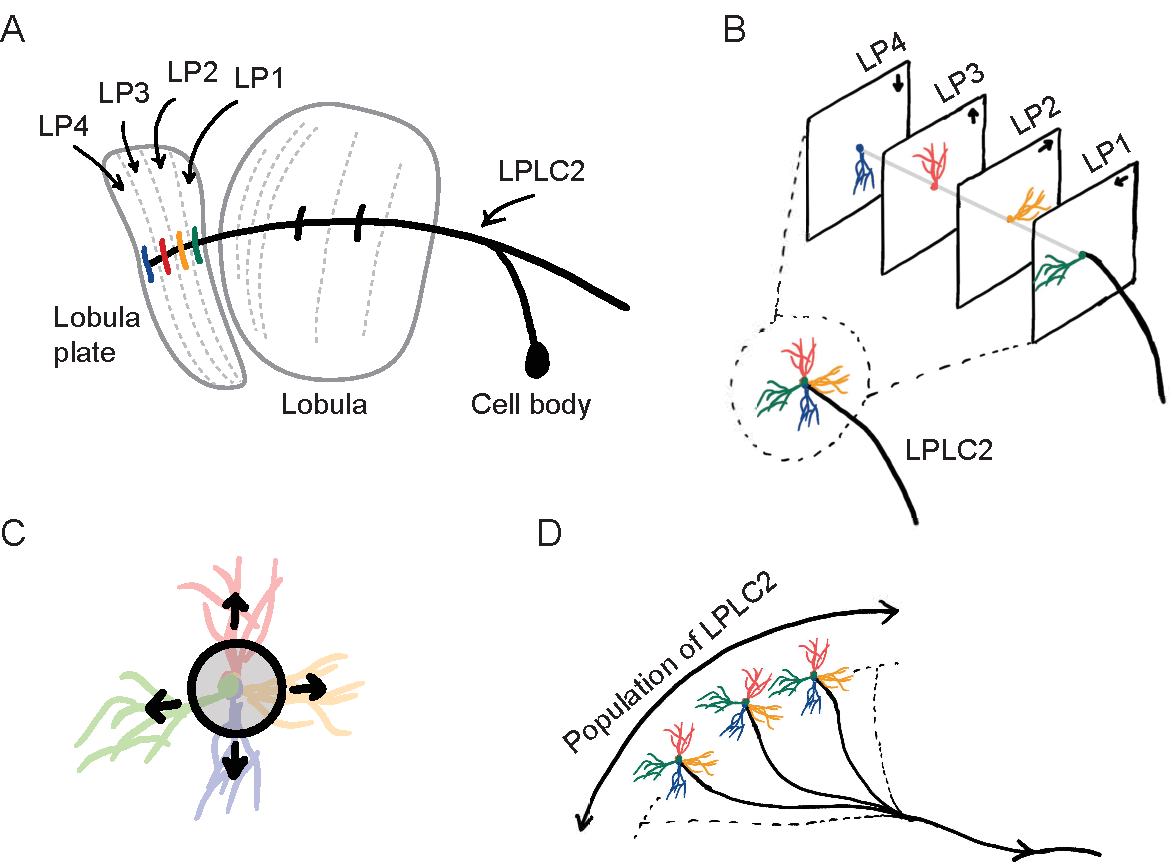
\includegraphics[width=\linewidth]{figures/anatomy_paper.pdf}
\caption{Sketches of the anatomical structures of LPLC2 neurons. (A) An LPLC2 neuron has dendrites in lobula and the four layers of the lobula plate (LP): LP1, LP2, LP3 and LP4. (B) The schematics of the four branches of the LPLC2 dendrites in the four layers of the LP. The arrows indicate the cardinal directions of the corresponding LP layers, which receive motion signals from motion detection neurons. (C) The outward dendritic structure of an LPLC2 neuron coincides with the expanding edges of a looming object (black circle). (D) A population of LPLC2 neurons (over 200) converge their axons to the giant fiber, a descending neuron, to contribute to escaping behaviors.}
\label{fig:anatomy}
\end{figure}

\begin{figure}
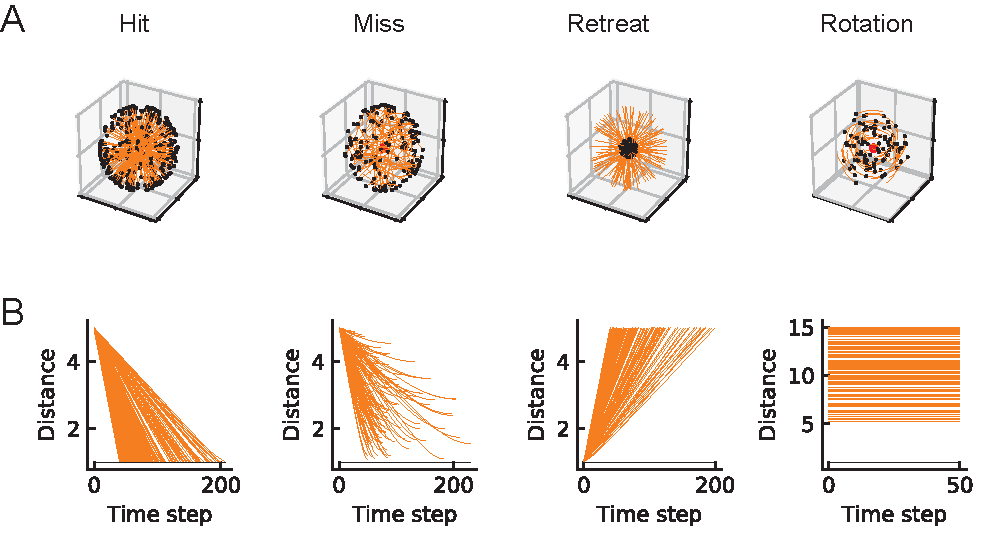
\includegraphics[width=\linewidth]{figures/stimuli_1_paper.pdf}
\caption{Four types of synthetic stimuli. (A) Orange lines represent trajectories of the stimuli. The black dots represent the starting points of the trajectories. For hit, miss, and retreat cases, multiple trajectories are shown. For rotation, only one trajectory is shown. (B) Distances of the objects to the fly eye as a function of time step.}
\label{fig:stimuli_traj}
%% If the optional argument in the square brackets is "none", then the caption *will not appear in the main figure at all* and only the full caption will appear under the supplementary figure at the end of the manuscript.
% \figsupp[Shorter caption for main text.]{This is a supplementary figure's full caption, which will be used at the end of the manuscript.}{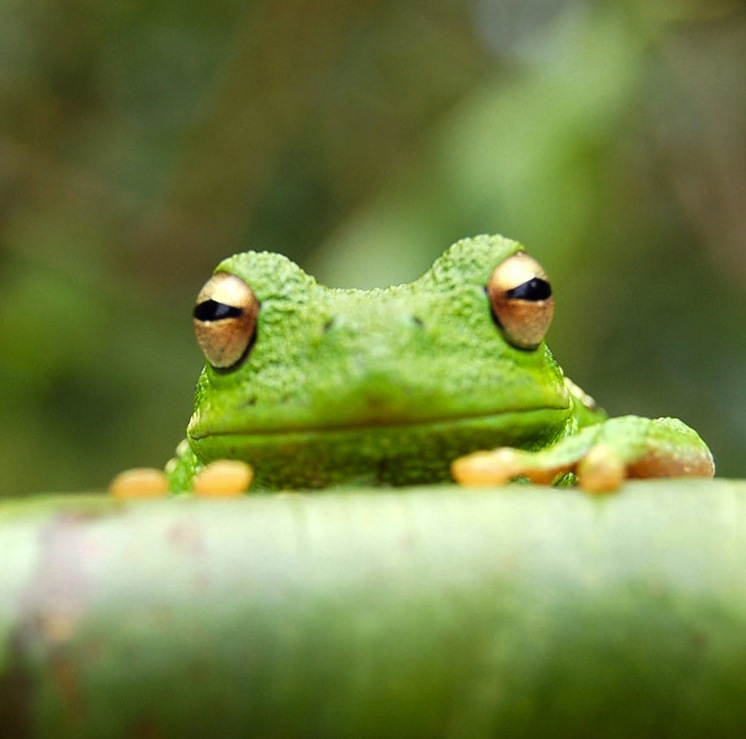
\includegraphics[width=6cm]{frog}}\label{figsupp:sf1}
% \figsupp{This is another supplementary figure.}{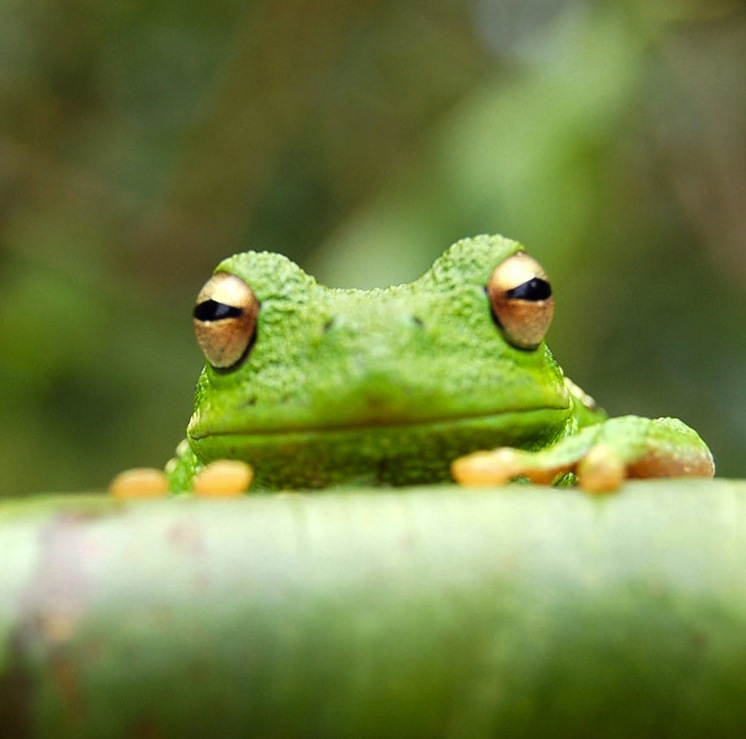
\includegraphics[width=6cm]{frog}}
% \videosupp{This is a description of a video supplement.}\label{videosupp:sv1}
% \figdata{This is a description of a data source.}\label{figdata:first}
% \figdata{This is another description of a data source.}\label{figdata:second}
\end{figure}

\begin{figure}
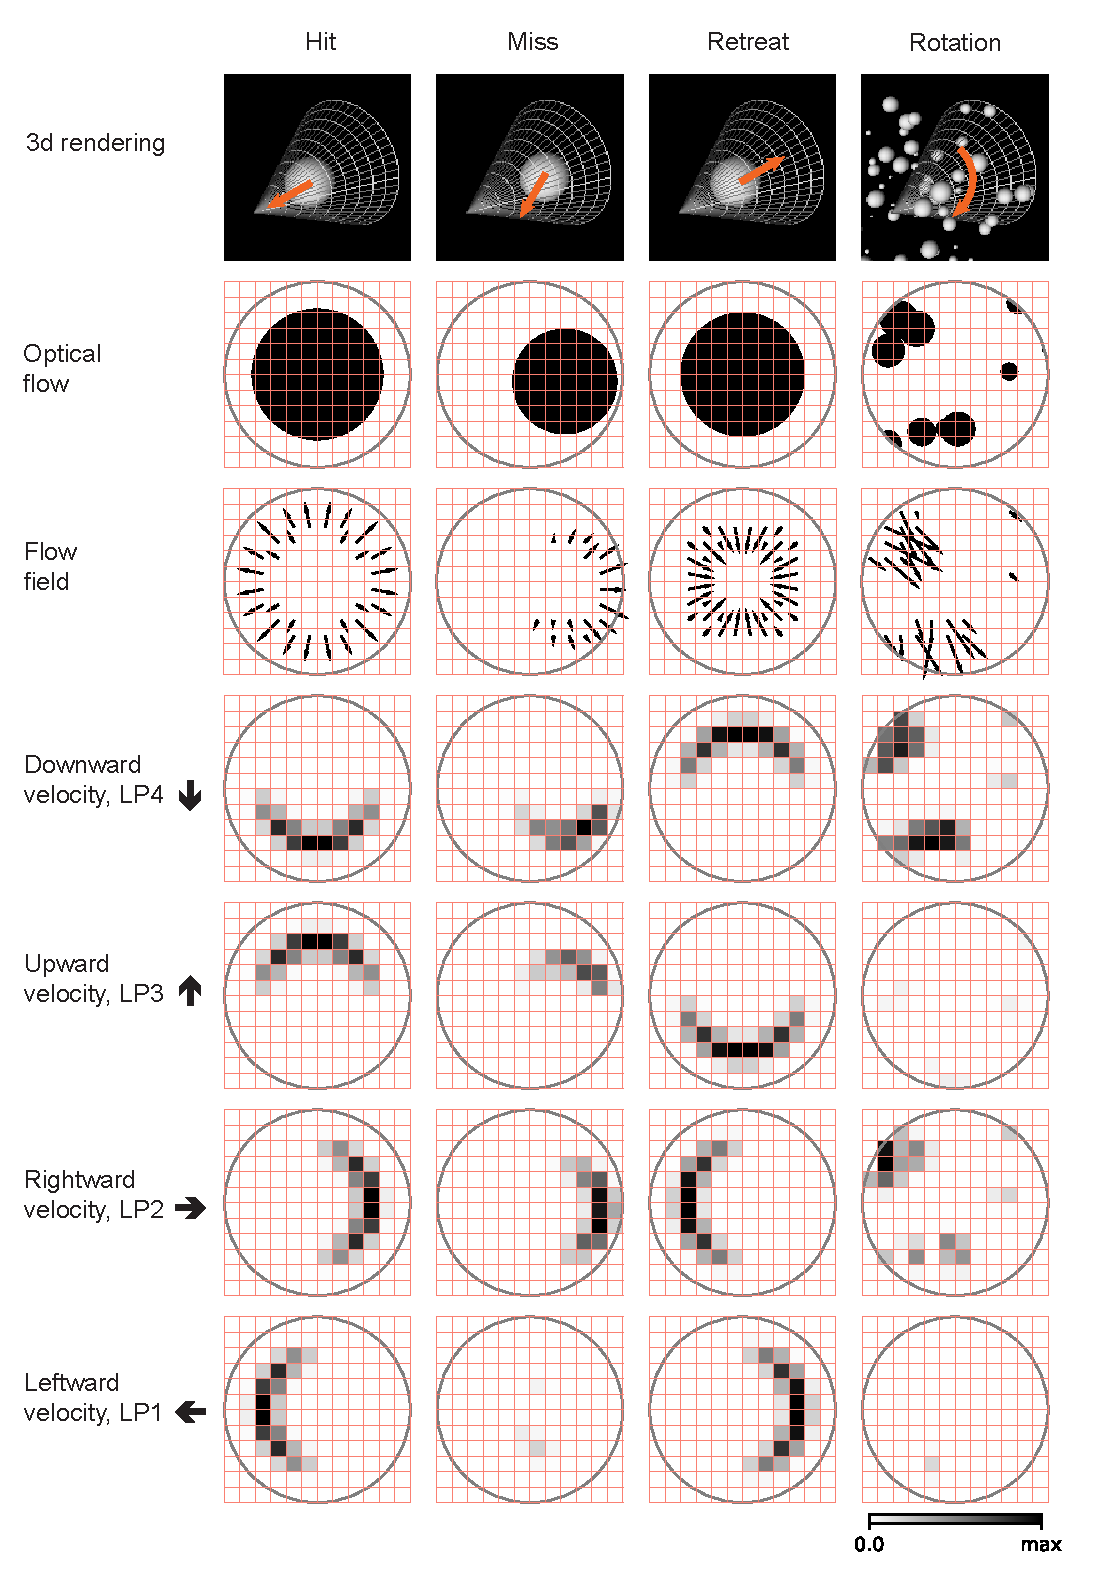
\includegraphics[width=\linewidth]{figures/stimuli_2_paper.pdf}
\caption{Corresponding to Fig. \ref{fig:stimuli_traj}), snapshots of optical flows and flow fields calculated by a Hassenstein Reichardt correlator (HRC) model. First row: 3d rendering of the spherical objects and the LPLC2 receptive field (the cones) at a specific time step. The orange arrows indicate the moving directions of the objects. Second row: 2d projections of the objects (black shades) within the LPLC2 receptive field (the grey circles). Third row: the thin black arrows indicate flow fields generated by the edges of the moving objects. Forth to seventh rows: decomposition of the flow fields in the four cardinal directions with respect to the LPLC2 neuron under consideration: downward, upward, rightward, and leftward, as indicated by the thick black arrows.}
\label{fig:stimuli_flow}
%% If the optional argument in the square brackets is "none", then the caption *will not appear in the main figure at all* and only the full caption will appear under the supplementary figure at the end of the manuscript.
% \figsupp[Shorter caption for main text.]{This is a supplementary figure's full caption, which will be used at the end of the manuscript.}{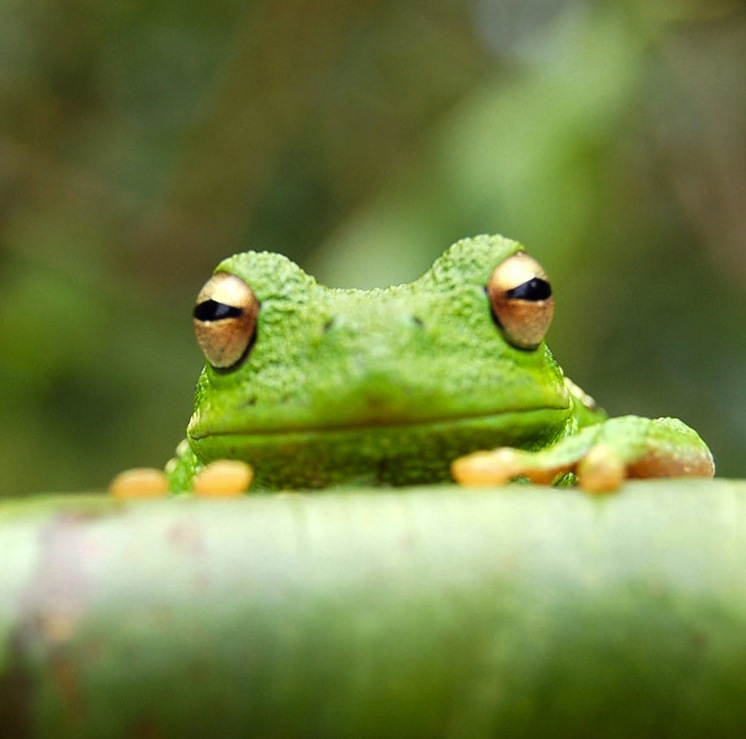
\includegraphics[width=6cm]{frog}}\label{figsupp:sf1}
% \figsupp{This is another supplementary figure.}{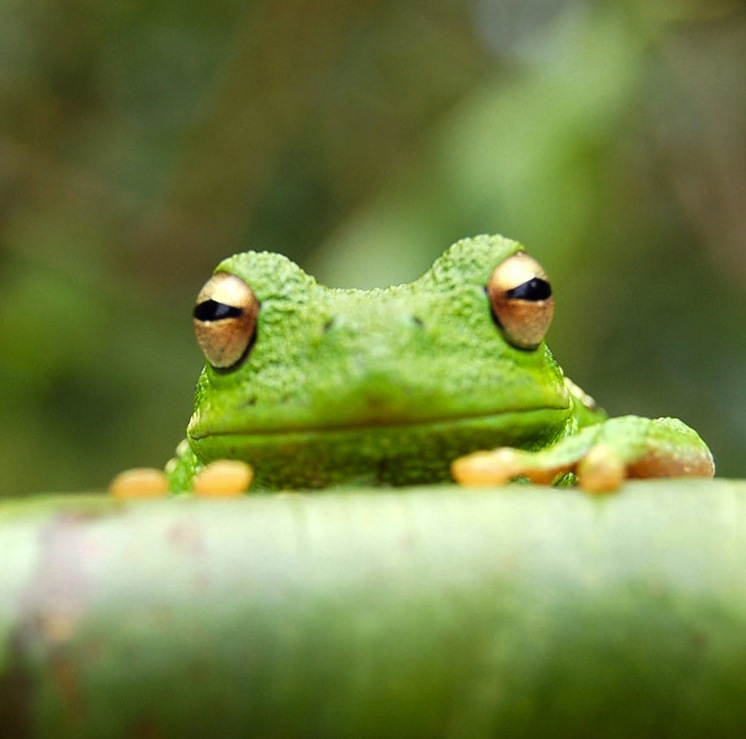
\includegraphics[width=6cm]{frog}}
% \videosupp{This is a description of a video supplement.}\label{videosupp:sv1}
% \figdata{This is a description of a data source.}\label{figdata:first}
% \figdata{This is another description of a data source.}\label{figdata:second}
\end{figure}

\begin{figure}
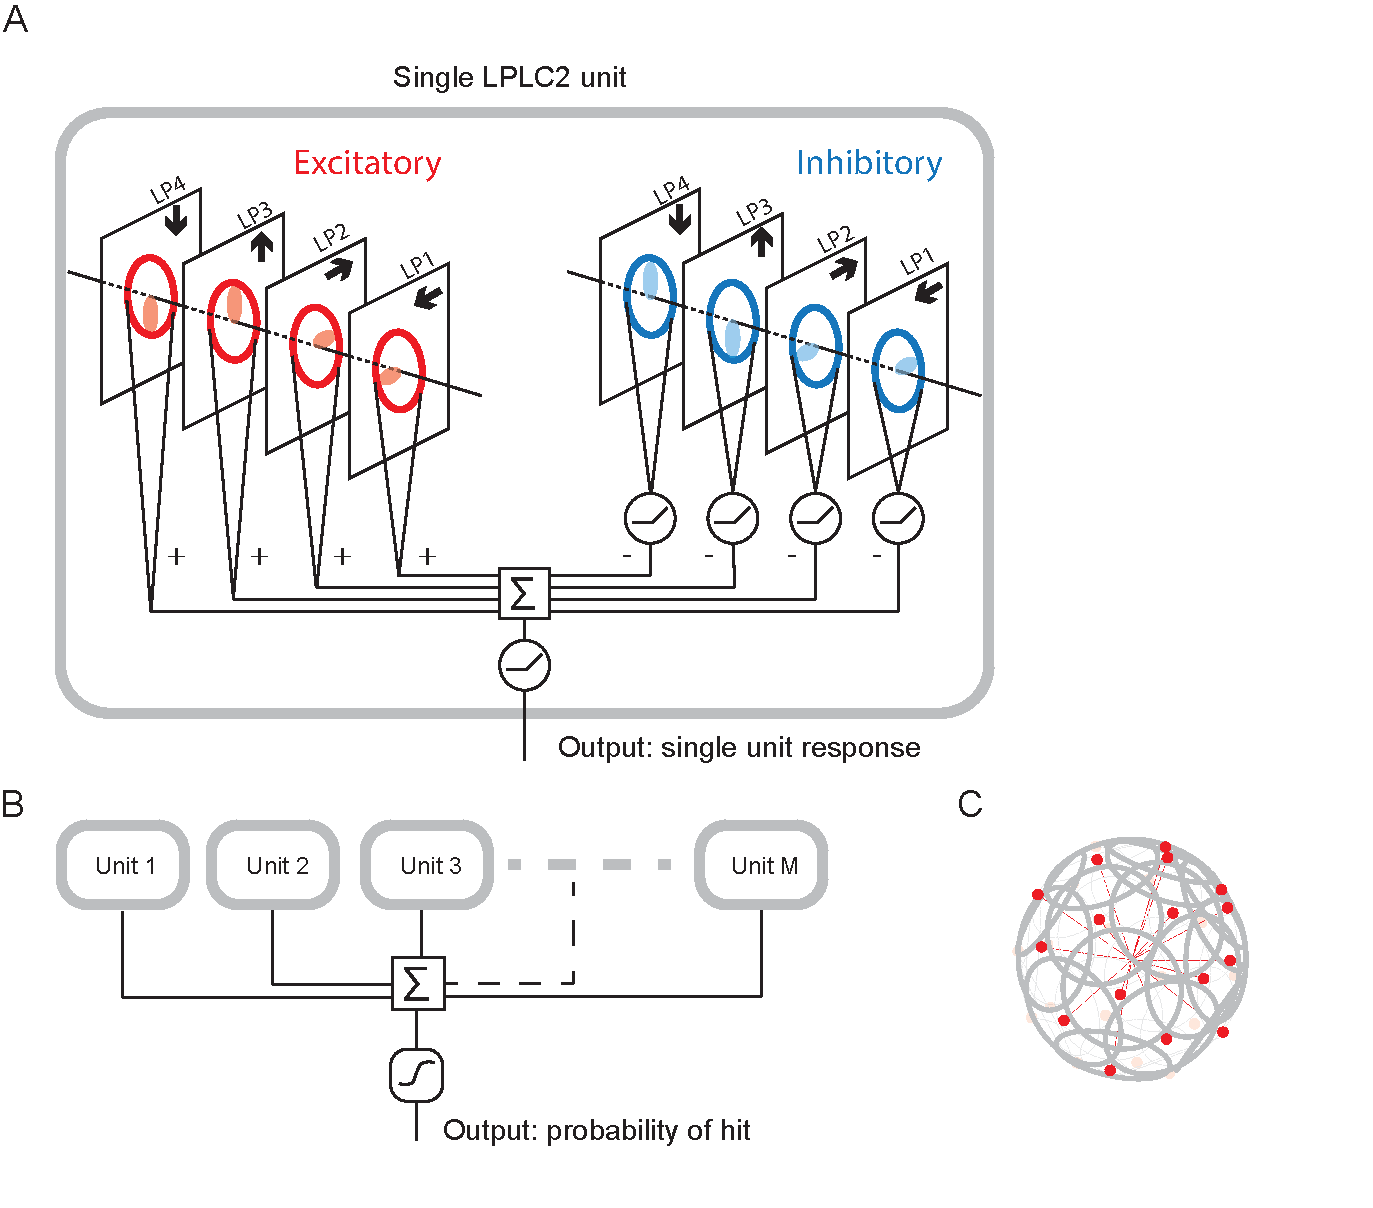
\includegraphics[width=\linewidth]{figures/model_sketch_paper.pdf}
\caption{Schematic of the model. (A) Single LPLC2 unit. There are two sets of nonnegative filters: excitatory (red) and inhibitory (blue). Each sets of filters have four branches, and each branch receives motion signals (forth to seventh rows in Fig. \ref{fig:stimuli_flow}) from the corresponding layer of the LP. The integrated signals from the excitatory branches and the inhibitory branches (rectified) are pooled together to go through a rectifier to produce an output, which is the response of a single LPLC2 unit. Each inhibitory input goes through a rectifier before pooled. (B) The outputs from $M$ LPLC2 units are summed and fed into a sigmoid function to estimate the probability of hit. (C) The $M$ LPLC2 units have their orientations almost evenly distributed in the angular space. Red dots and lines represent the centers of the receptive fields and the grey lines represent the boundaries of the receptive fields.}
\label{fig:model}
%% If the optional argument in the square brackets is "none", then the caption *will not appear in the main figure at all* and only the full caption will appear under the supplementary figure at the end of the manuscript.
% \figsupp[Shorter caption for main text.]{This is a supplementary figure's full caption, which will be used at the end of the manuscript.}{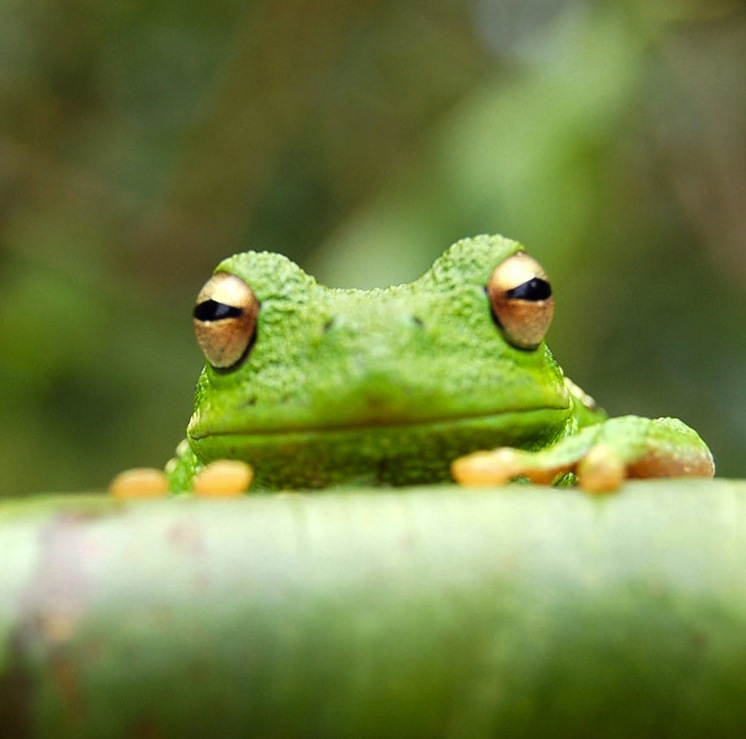
\includegraphics[width=6cm]{frog}}\label{figsupp:sf1}
% \videosupp{This is a description of a video supplement.}\label{videosupp:sv1}
% \figdata{This is a description of a data source.}\label{figdata:first}
% \figdata{This is another description of a data source.}\label{figdata:second}
\end{figure}

\begin{figure}
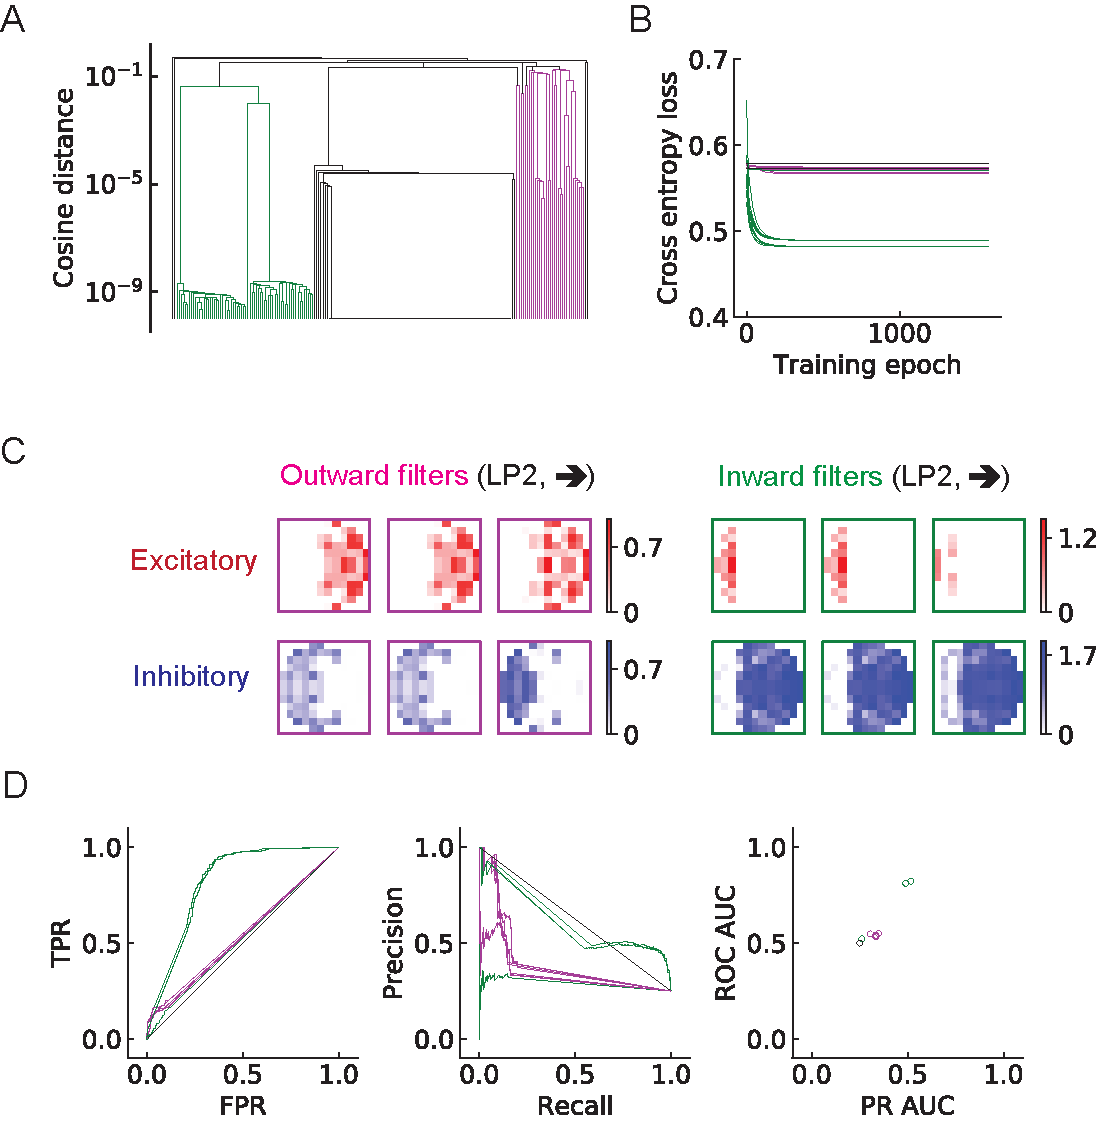
\includegraphics[width=\linewidth]{figures/trained_results_Q1_paper.pdf}
\caption{Two distinct types of models appear from training a single LPLC2 unit on the binary classification task. (A) Clustering of the trained filters/weights shown as a dengrogram. Different colors indicate different clusters, which are preserved for the rest of the paper. (B) The trajectories of the loss functions during training. (C) The two distinct types of models are represented by two types of filters that are exactly the opposite to each other: outward model (magenta) and inward model (green). The excitatory filters are shown as red, and the inhibitory filters are shown as blue. (D) Performances of the two models. TPR: true positive rate; FPR: false positive rate; ROC: receiver operating characteristic; PR: precision recall; AUC: area under the curve.}
\label{fig:trained_res_singlecell}
%% If the optional argument in the square brackets is "none", then the caption *will not appear in the main figure at all* and only the full caption will appear under the supplementary figure at the end of the manuscript.
\figsupp[More examples of the trained filters for the two types of models and the inferred probability of hit for the four types synthetic stimuli.]{(A) Trained filters: outward model (magenta) and inward model (green). (B) Probability of hit inferred by a single LPLC2 unit for the four types synthetic stimuli.}{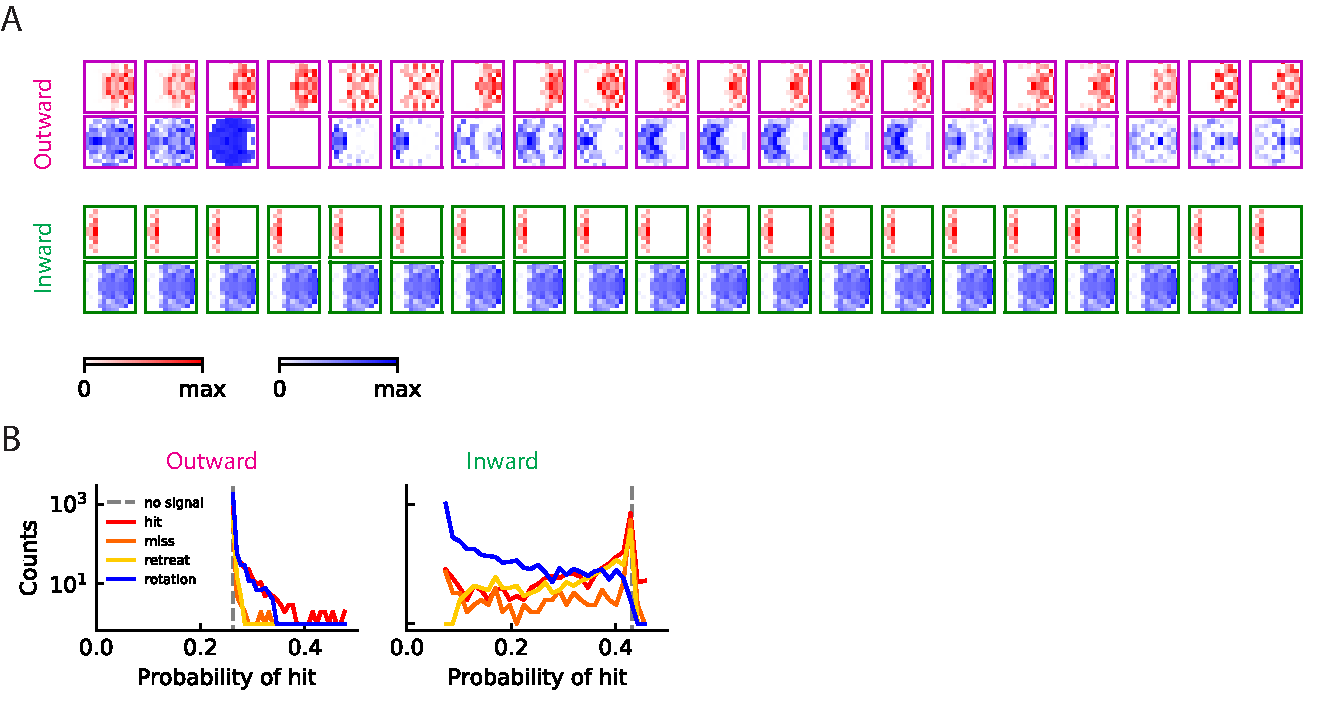
\includegraphics[width=\linewidth]{sup_figures/trained_results_Q1_sup_paper.pdf}}\label{figsupp:sf1_trained_res_singlecell}
% \figsupp{This is another supplementary figure.}{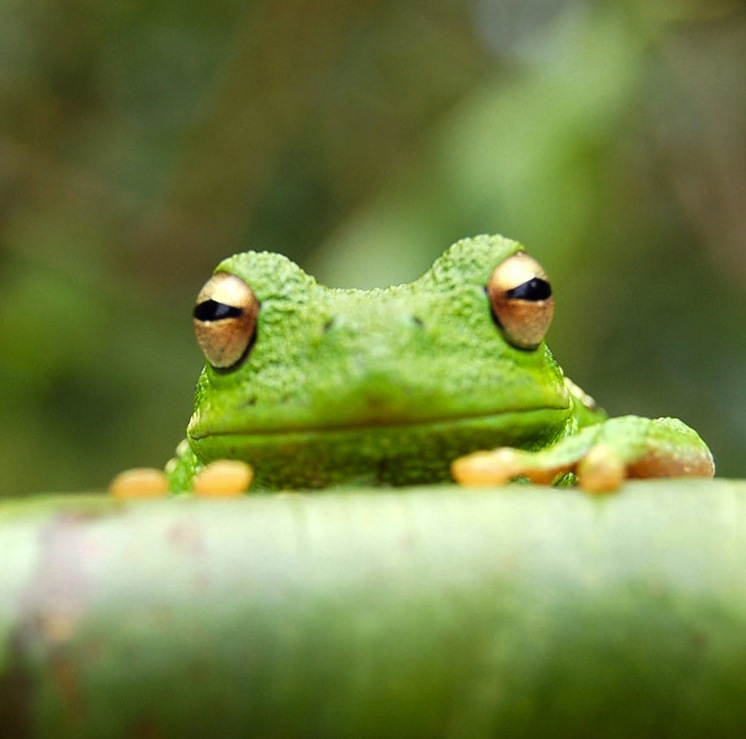
\includegraphics[width=6cm]{frog}}
% \videosupp{This is a description of a video supplement.}\label{videosupp:sv1}
% \figdata{This is a description of a data source.}\label{figdata:first}
% \figdata{This is another description of a data source.}\label{figdata:second}
\end{figure}

\begin{figure}
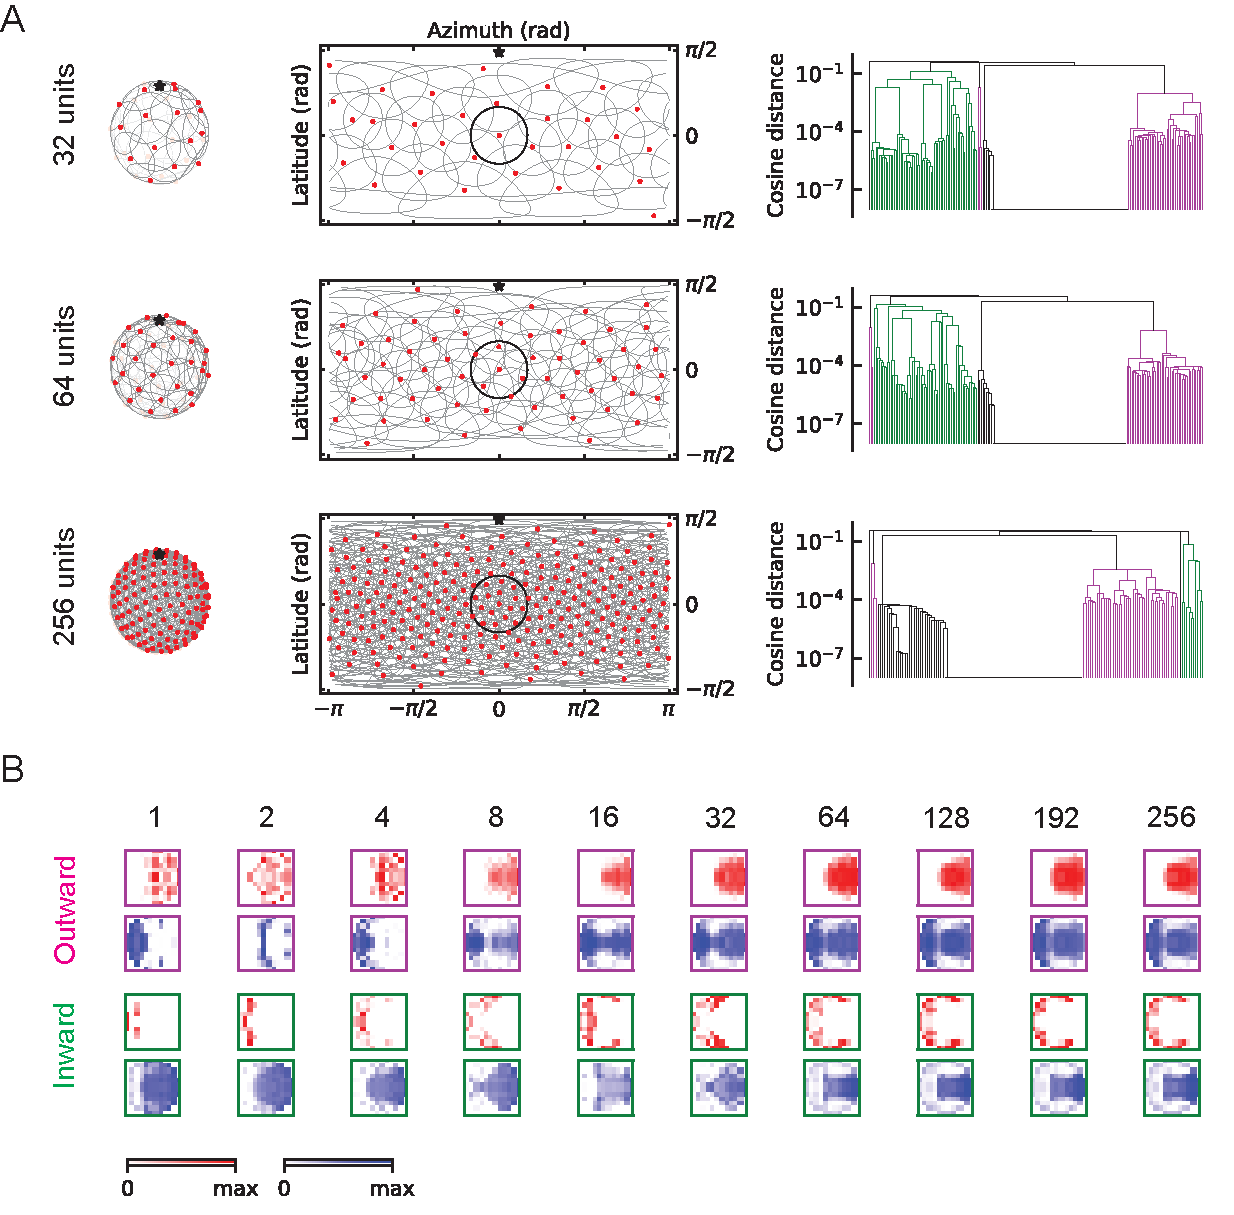
\includegraphics[width=\linewidth]{figures/trained_results_multicells_paper.pdf}
\caption{The outward and inward models also appear for models with multiple LPLC2 units. (A) Left column: angular distributions of the LPLC2 units, where red dots are centers of the receptive fields, the grey circles are the boundaries of the receptive field and the black star shows the top of the fly head. Middle column: 2d mapping of the LPLC2 units with symbols being the same as in the left column. Right column: clustering results shown as dendrogams with color codes the same as in Fig. \ref{fig:trained_res_singlecell}A). (B) Examples of the trained excitatory/inhibitory filters for outward and inward models with different numbers of LPLC2 units.}
\label{fig:trained_res_multicells}
%% If the optional argument in the square brackets is "none", then the caption *will not appear in the main figure at all* and only the full caption will appear under the supplementary figure at the end of the manuscript.
\figsupp[Performance of the models.]{Same as in Fig. \ref{fig:trained_res_singlecell}D) but for models with multiple LPLC2 units.}{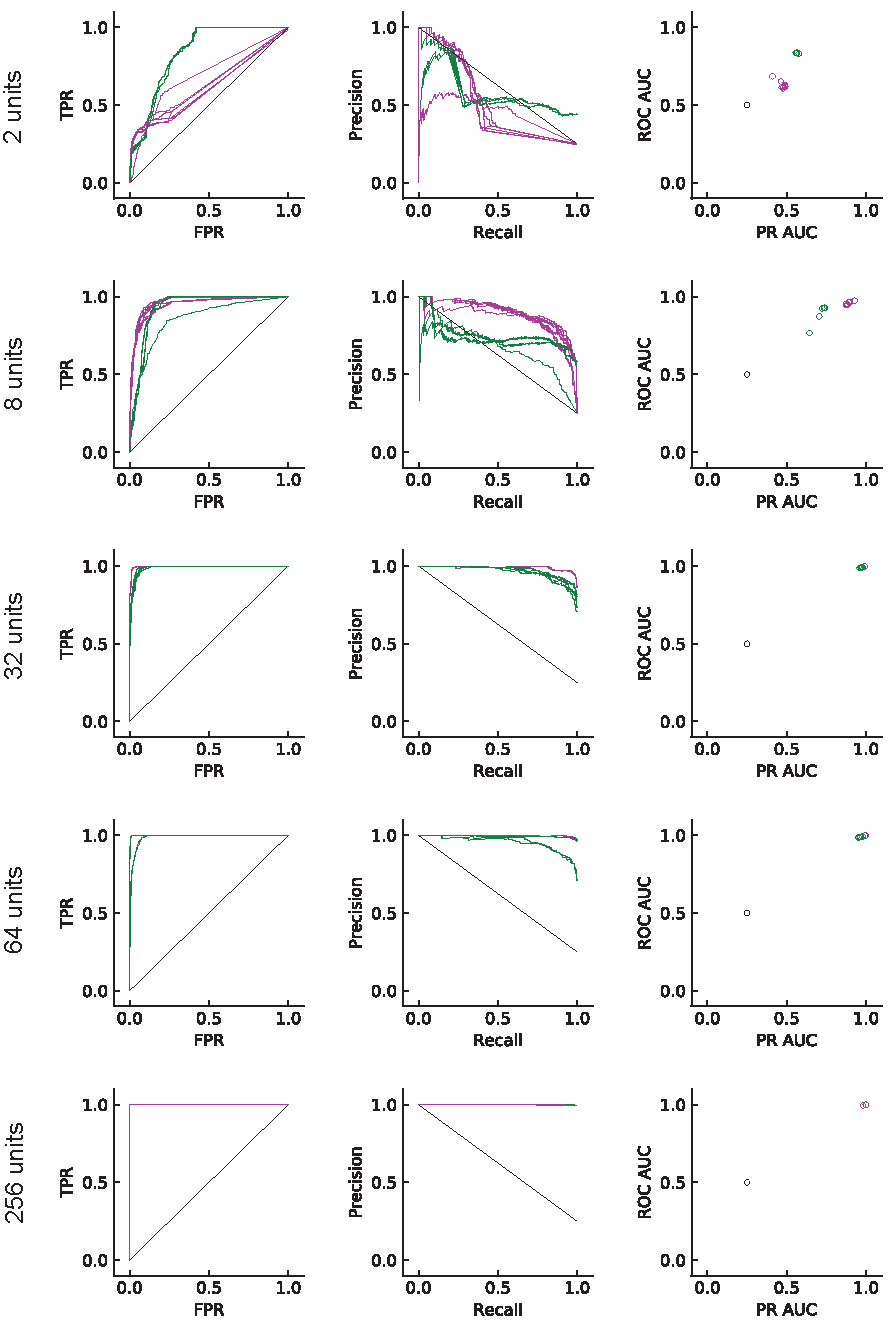
\includegraphics[width=\linewidth]{sup_figures/trained_results_multicells_sup1_paper.pdf}}\label{figsupp:sf1_trained_res_multicells}
\figsupp[More examples of the outward filters.]{}{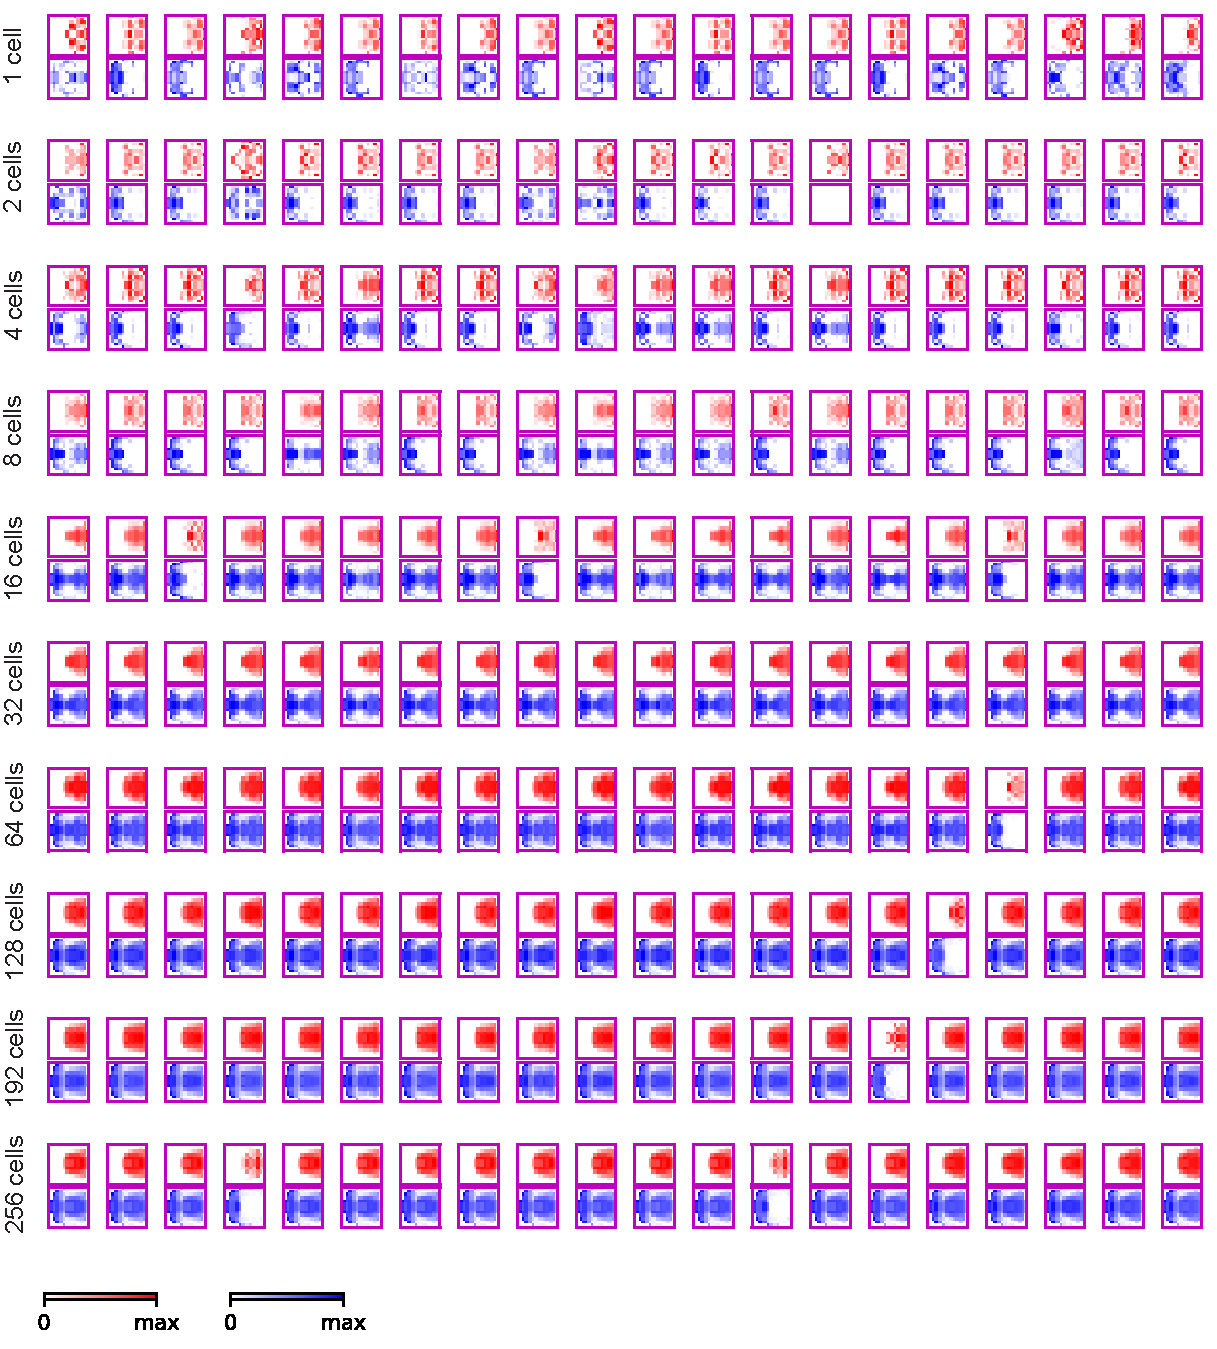
\includegraphics[width=\linewidth]{sup_figures/trained_results_multicells_sup2_paper.pdf}}\label{figsupp:sf2_trained_res_multicells}
\figsupp[More examples of the inward filters.]{}{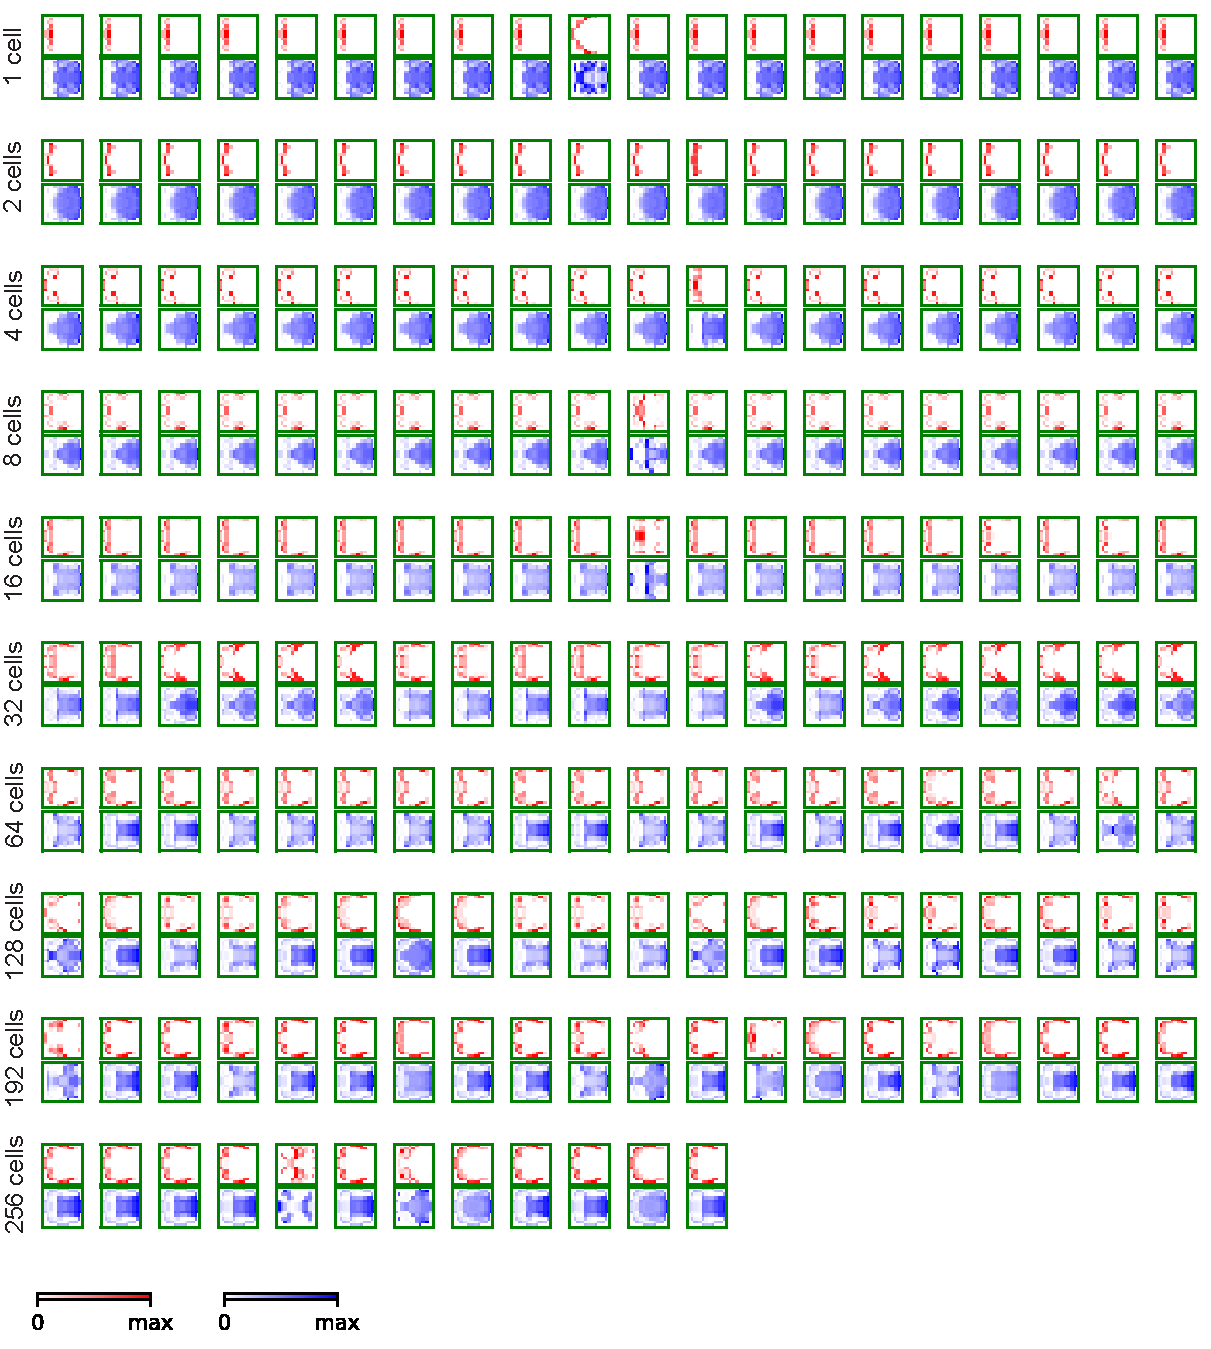
\includegraphics[width=\linewidth]{sup_figures/trained_results_multicells_sup3_paper.pdf}}\label{figsupp:sf3_trained_res_multicells}
% \videosupp{This is a description of a video supplement.}\label{videosupp:sv1}
% \figdata{This is a description of a data source.}\label{figdata:first}
% \figdata{This is another description of a data source.}\label{figdata:second}
\end{figure}

\begin{figure}
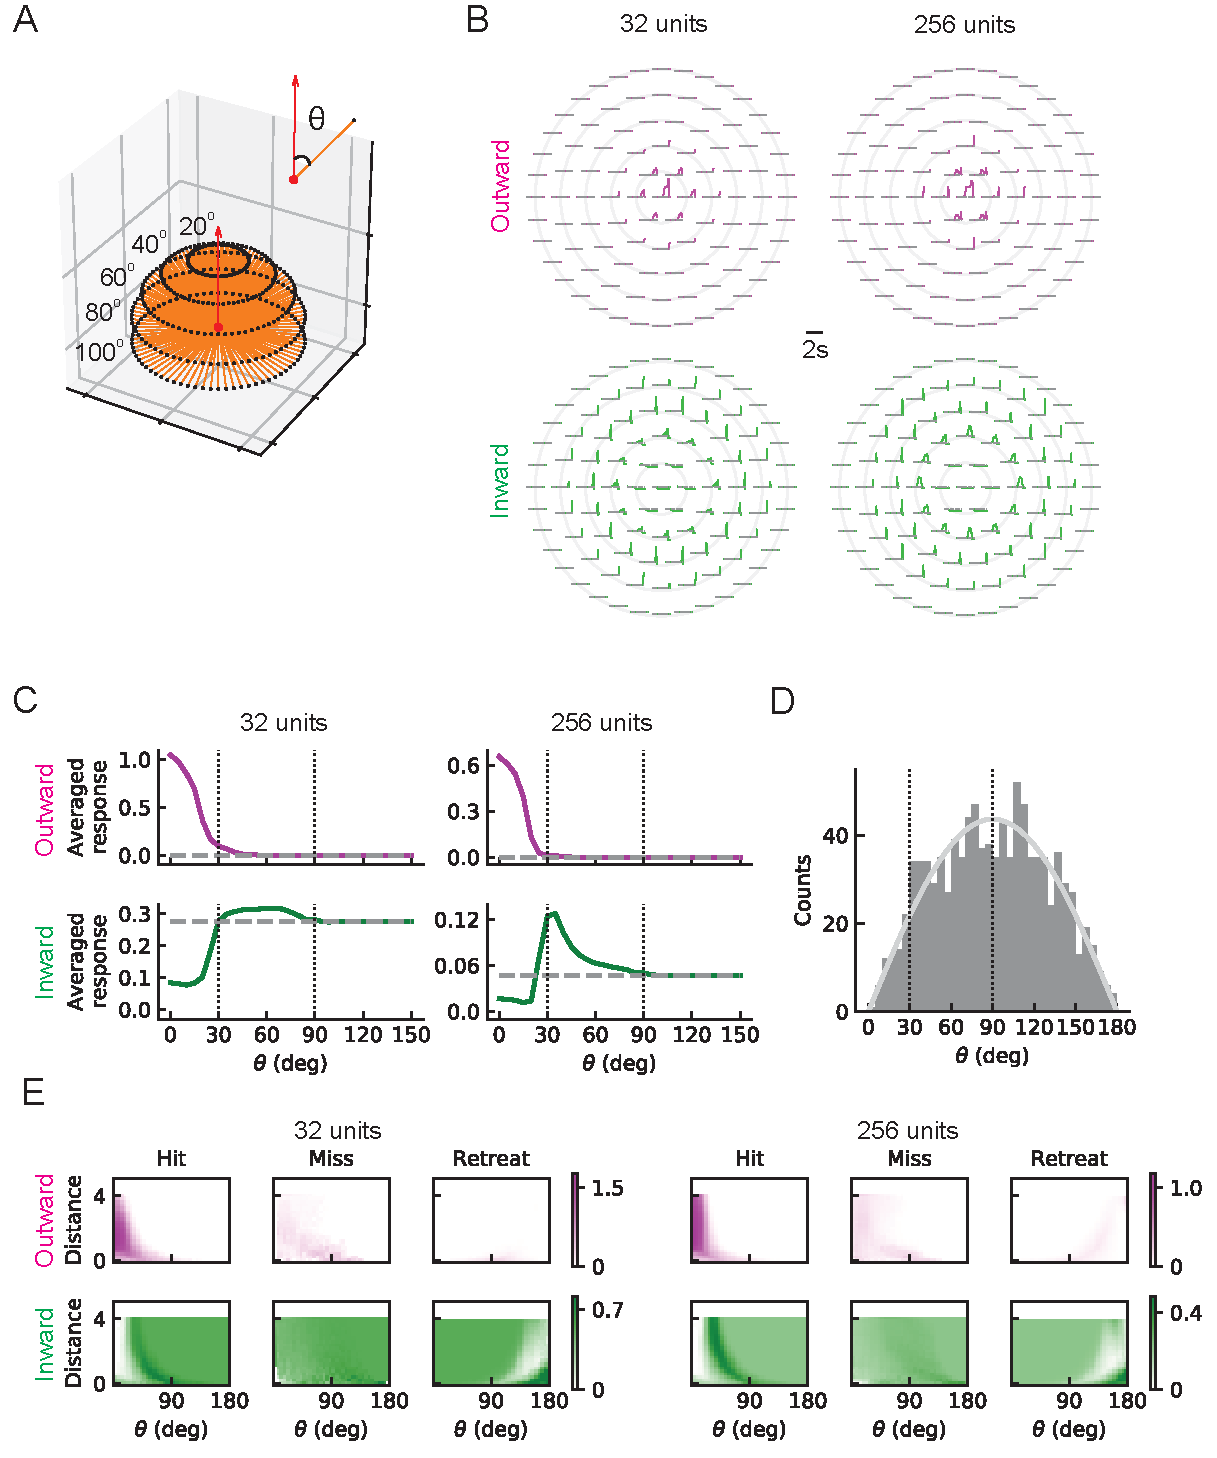
\includegraphics[width=\linewidth]{figures/compare_outward_inward_single_unit_paper.pdf}
\caption{The outward and inward filters show distinct behaviors: single unit analysis. (A) Trajectories of hit stimuli with different incoming angles $\theta$. Symbols are the same as in Fig. \ref{fig:stimuli_traj}) except that the upward red arrow represents the orientation of one LPLC2 unit. The numbers with degree unit indicate the specific values of the incoming angles. (B) Response patterns of a single LPLC2 unit with either outward (magenta) or inward (green) filters obtained from models with 32 and 256 units, respectively. The grey dashed lines show the baseline activity of the unit when there is no stimulus. The solid grey concentric circles correspond to the values of the incoming angles in (A). (C) Temporally averaged responses against the incoming angle $\theta$. Symbols and color codes are the same as in (B). (D) Histogram of the incoming angles for the hit stimuli in Fig. \ref{fig:stimuli_traj}A). The grey curve represents a rescaled sine wave with half of the period. (E) Heatmaps of the responses of a single LPLC2 unit against the incoming angle $\theta$ and the distance to the fly head, for both outward and inward filters obtained from models with 32 and 256 units, respectively.}
\label{fig:compare_single}
%% If the optional argument in the square brackets is "none", then the caption *will not appear in the main figure at all* and only the full caption will appear under the supplementary figure at the end of the manuscript.
% \figsupp[Shorter caption for main text.]{This is a supplementary figure's full caption, which will be used at the end of the manuscript.}{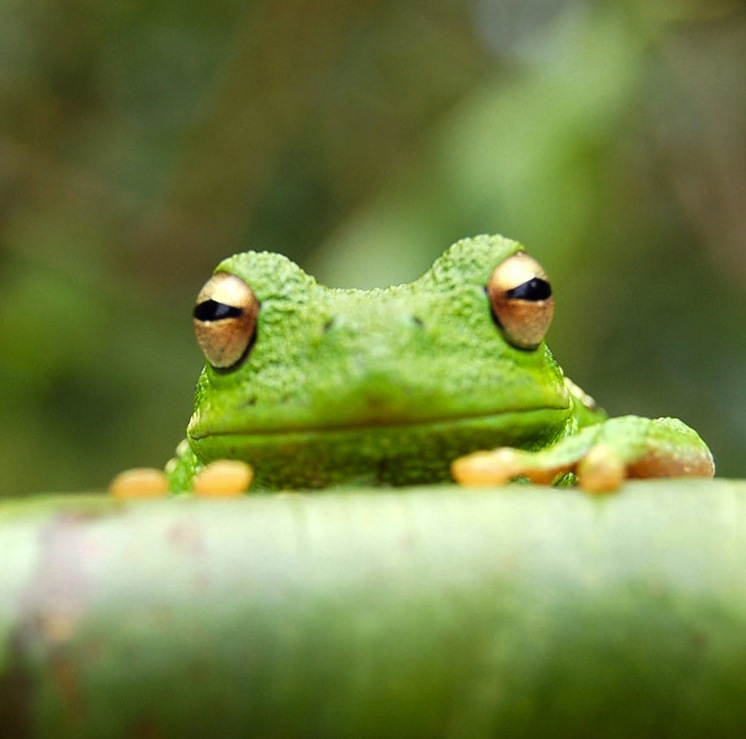
\includegraphics[width=6cm]{frog}}\label{figsupp:sf1}
% \figsupp{This is another supplementary figure.}{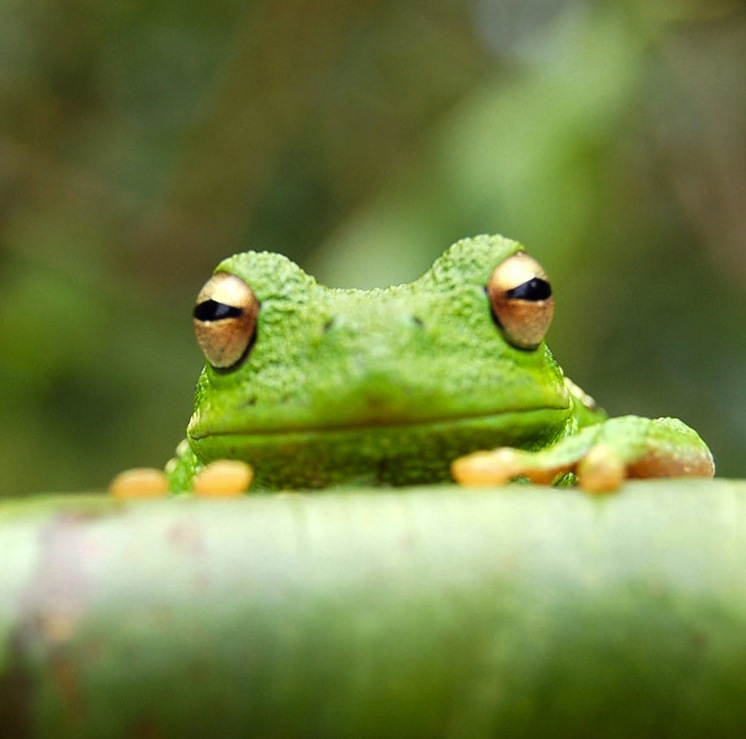
\includegraphics[width=6cm]{frog}}
% \videosupp{This is a description of a video supplement.}\label{videosupp:sv1}
% \figdata{This is a description of a data source.}\label{figdata:first}
% \figdata{This is another description of a data source.}\label{figdata:second}
\end{figure}

\begin{figure}
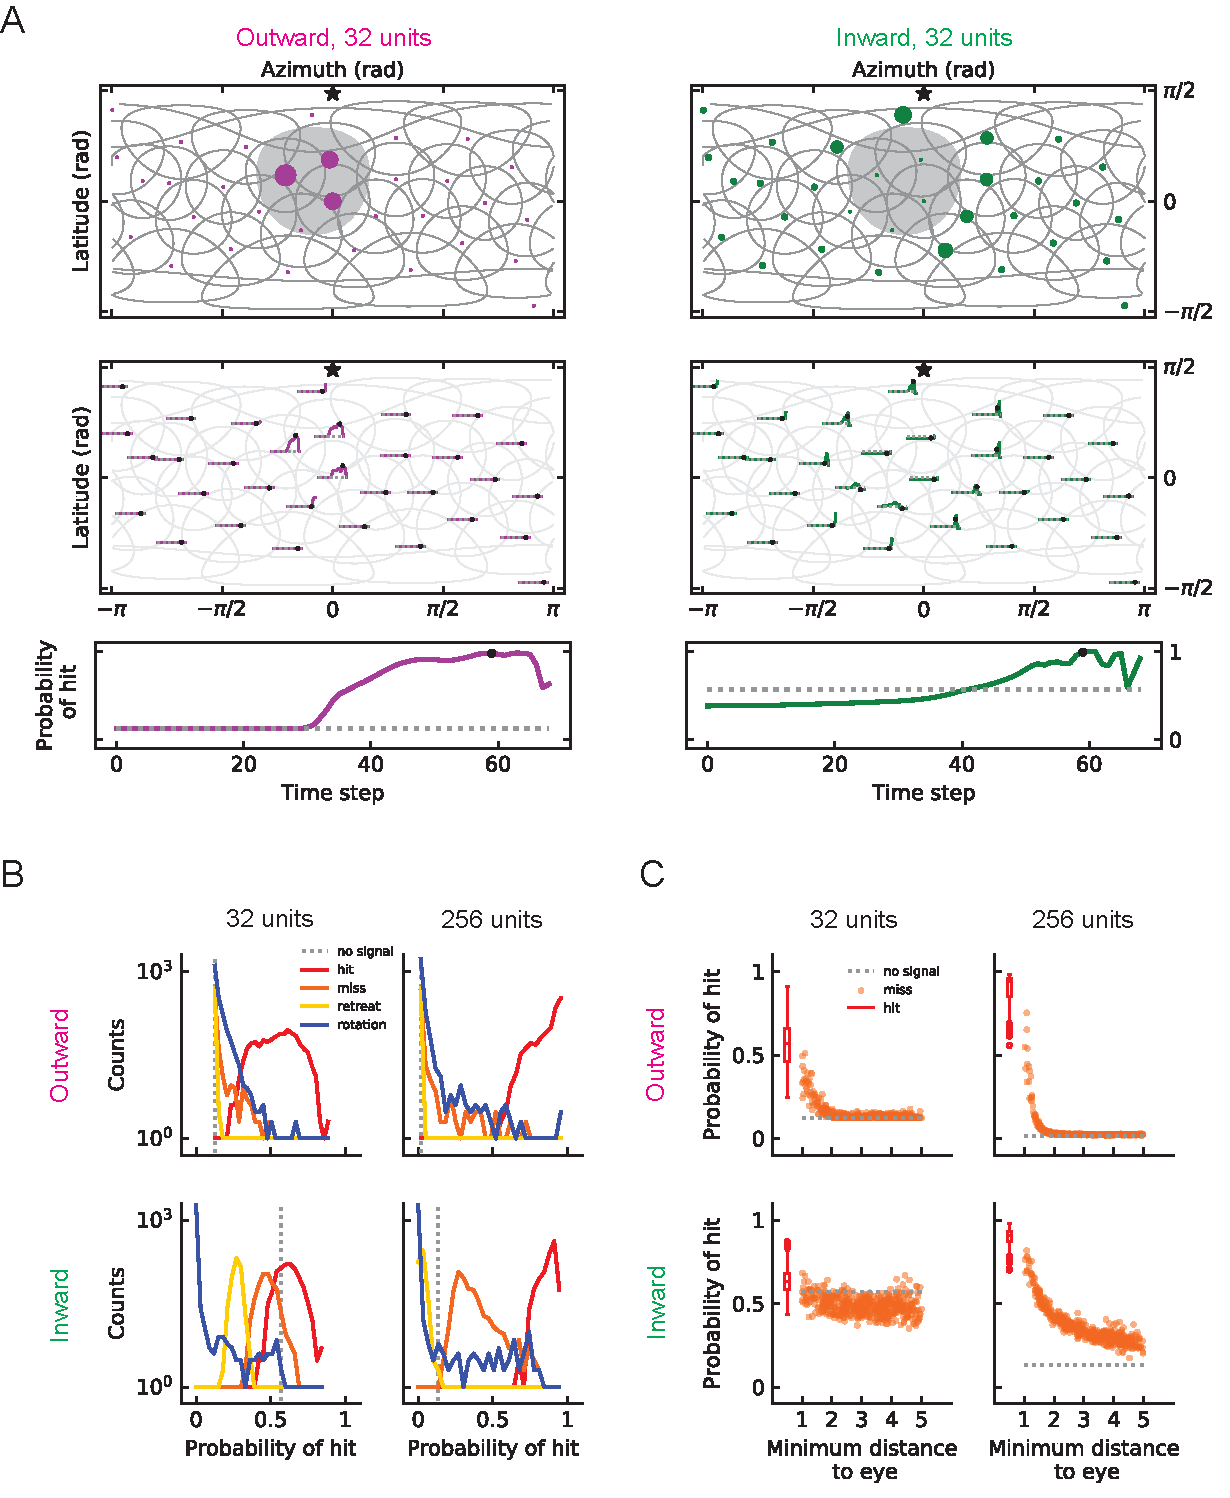
\includegraphics[width=\linewidth]{figures/compare_outward_inward_multiple_units_paper.pdf}
\caption{Population coding. (A) Top row: a snapshot of the responses of the outward LPLC2 units (magenta dots) for a hitting object (grey shade). Symbols and color codes are the same as in Fig. \ref{fig:trained_res_multicells}A). Middle row: the whole trajectories of the responses for the same hitting object as in the top row. Bottom row: the whole trajectories of the probability of hit for the same hitting object as in the top row. (B) Histograms of the probability of hit inferred by models with 32 or 256 LPLC2 units for the four types of synthetic stimuli. (C) The inferred probability of hit as a function of the minimum distance of the object to the fly eye for the miss cases.}
\label{fig:compare_multi}
%% If the optional argument in the square brackets is "none", then the caption *will not appear in the main figure at all* and only the full caption will appear under the supplementary figure at the end of the manuscript.
\figsupp[The same as (A), but for miss and retreat stimuli.]{}{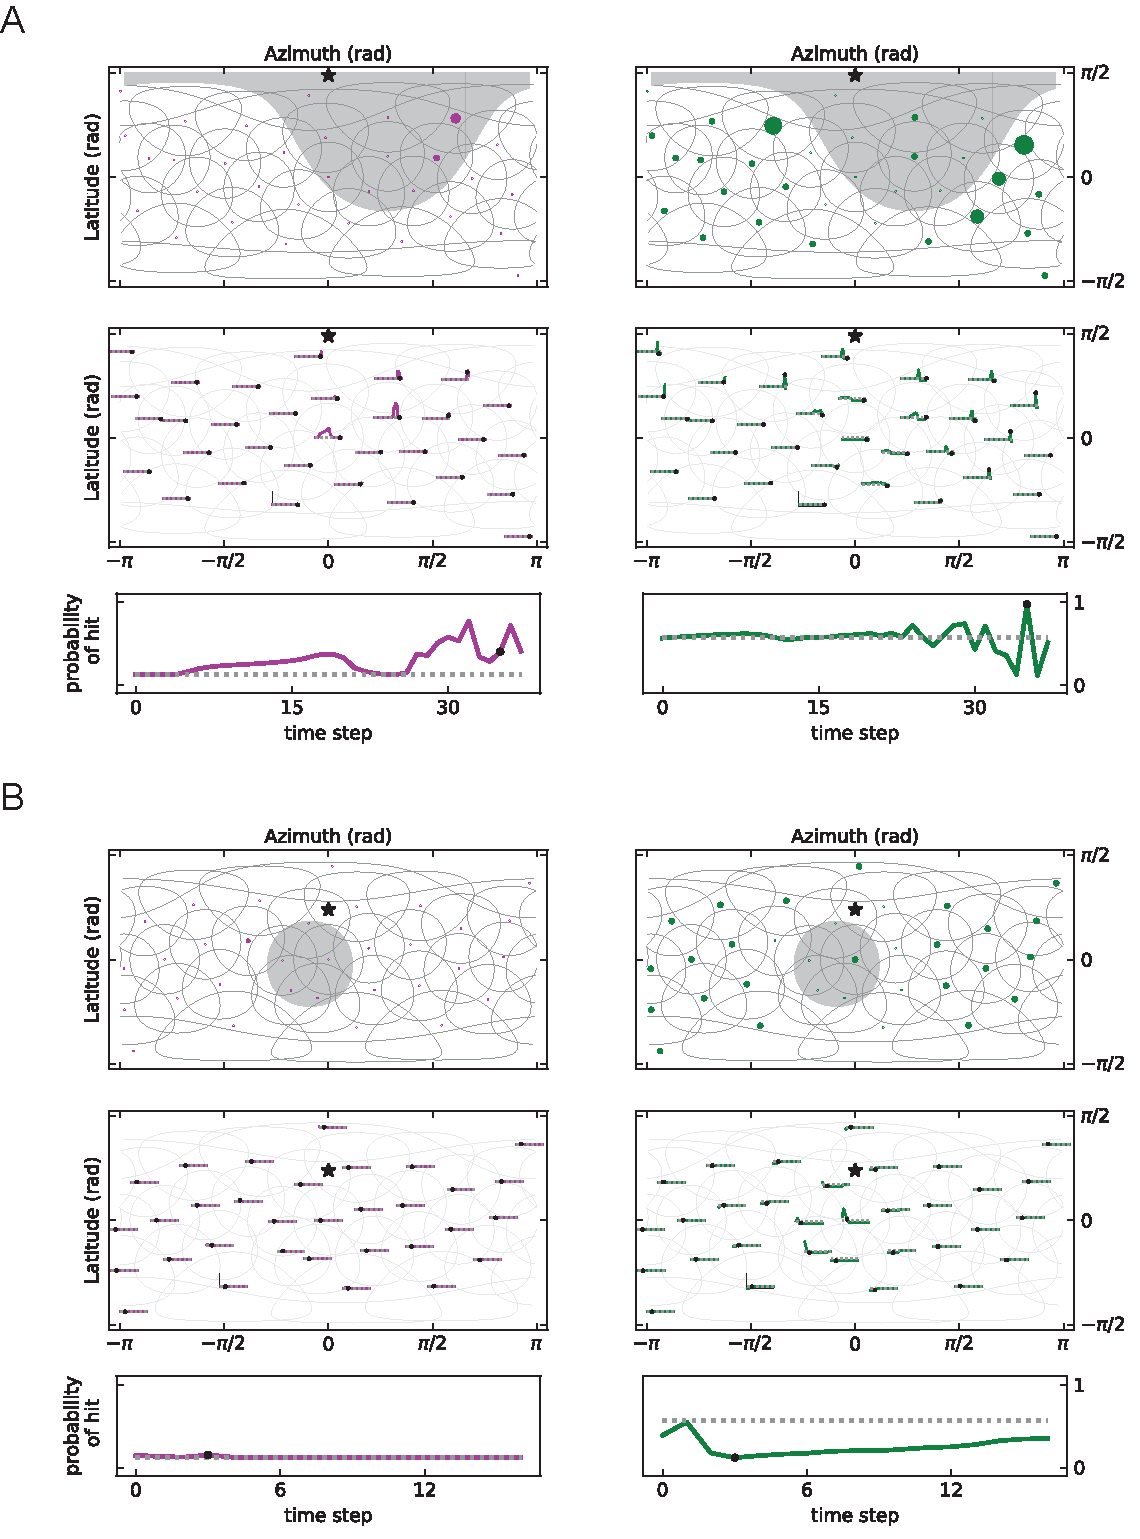
\includegraphics[width=\linewidth]{sup_figures/compare_outward_inward_multiple_units_sup_paper.pdf}}\label{figsupp:sf1_compare_multi}
% \figsupp{This is another supplementary figure.}{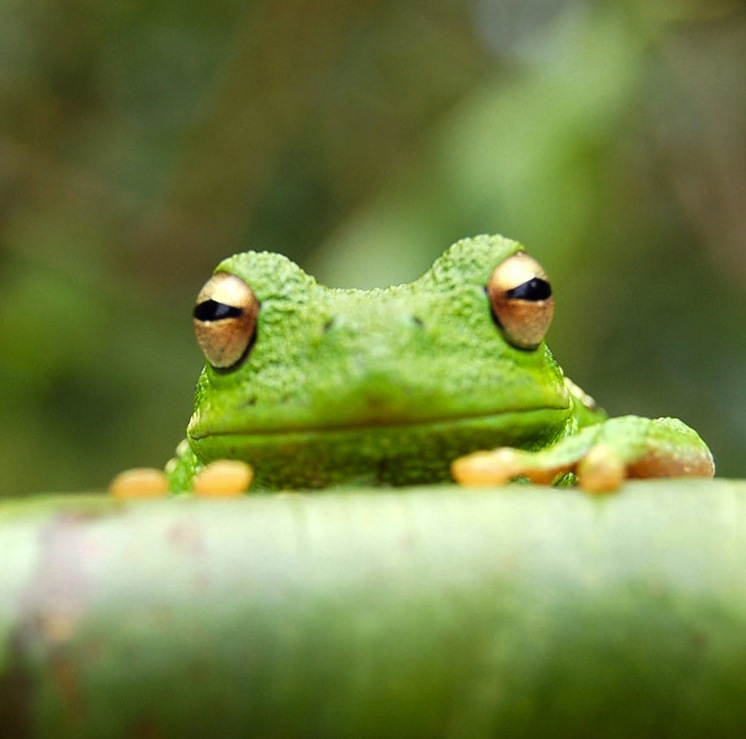
\includegraphics[width=6cm]{frog}}
% \videosupp{This is a description of a video supplement.}\label{videosupp:sv1}
% \figdata{This is a description of a data source.}\label{figdata:first}
% \figdata{This is another description of a data source.}\label{figdata:second}
\end{figure}

\begin{figure}
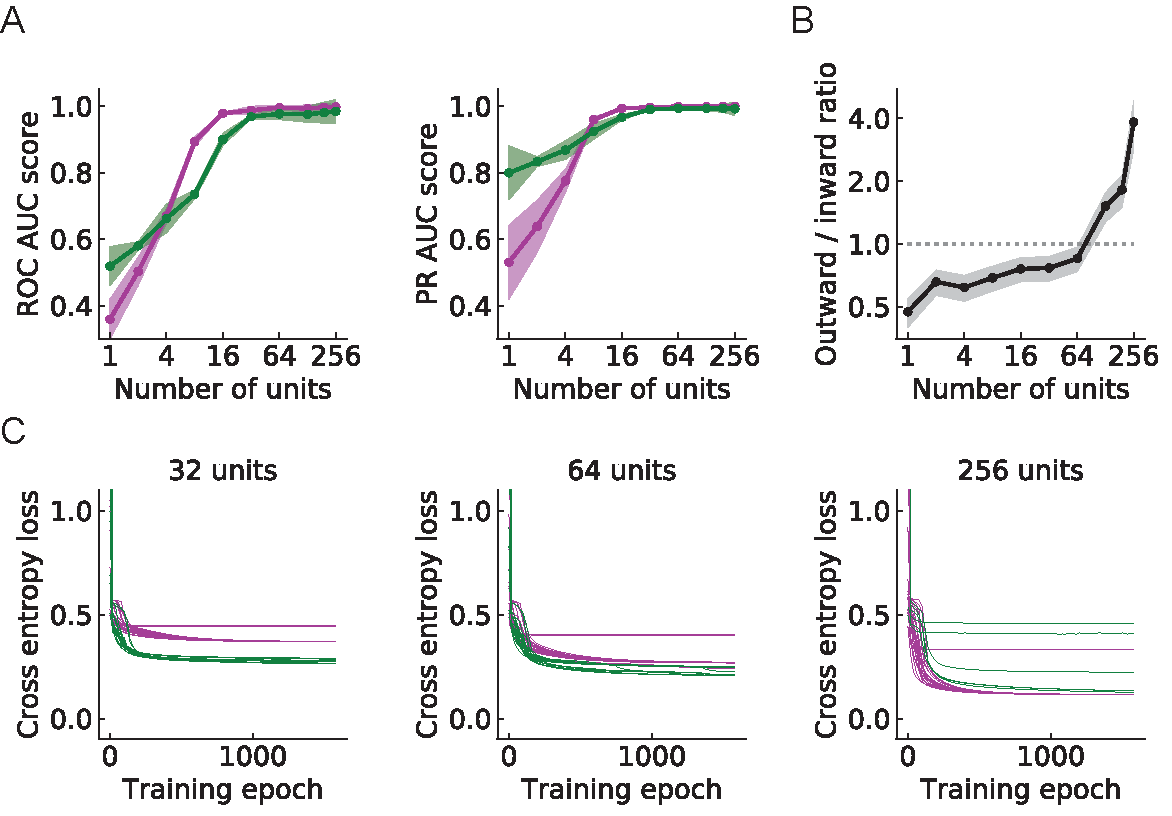
\includegraphics[width=\linewidth]{figures/outward_better_than_inward_paper.pdf}
\caption{Large populations of LPLC2 units improve performances and favor outward models. (A) Both ROC and PR AUC scores increase as the number of LPLC2 units increases. Lines and dots: average scores; shades: one standard deviation of the scores. Magenta: outward models; green: inward models. (B) The black line and dots show the ratio of the numbers of the two types of the models obtained by varying randomly the initial conditions of the training. The grey shades indicate one standard deviation obtained by assuming the training is a binomial event. The dotted horizontal line indicates the ratio of 1. (C) AS the population of LPLC2 units increase, cross entropy losses of the outward models become lower than the inward models.}
\label{fig:outward_prevail}
%% If the optional argument in the square brackets is "none", then the caption *will not appear in the main figure at all* and only the full caption will appear under the supplementary figure at the end of the manuscript.
\figsupp[Same as in (A) and (B) but for training in different conditions.]{(A) A different probability model (METHOD). (B) Training without rotation stimuli. (C) Training with larger distances of the objects to the fly eye.}{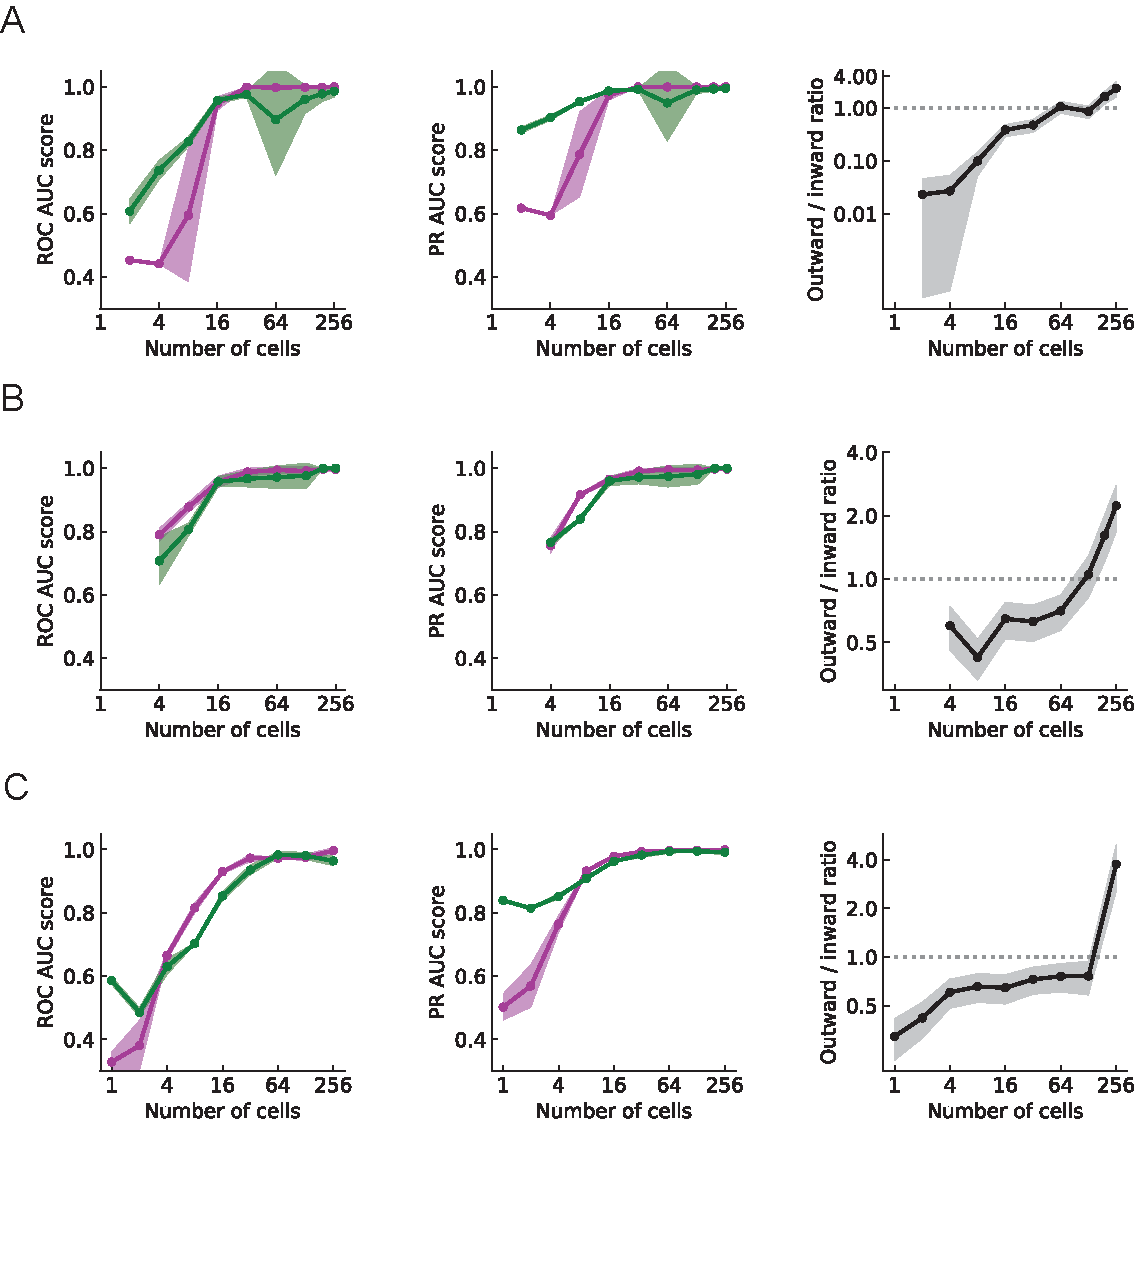
\includegraphics[width=\linewidth]{sup_figures/outward_better_than_inward_sup_paper.pdf}}\label{figsupp:sf1_outward_prevail}
% \figsupp{This is another supplementary figure.}{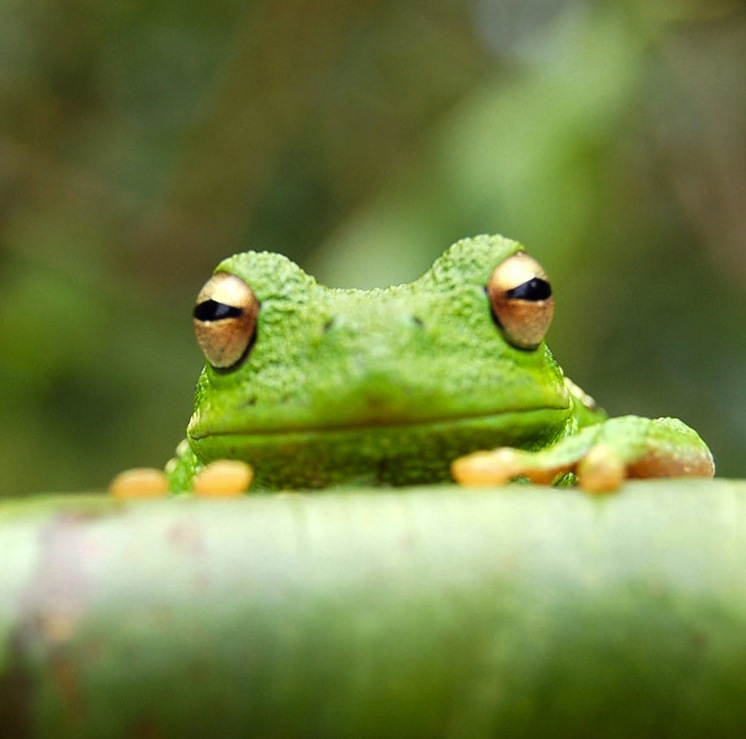
\includegraphics[width=6cm]{frog}}
% \videosupp{This is a description of a video supplement.}\label{videosupp:sv1}
% \figdata{This is a description of a data source.}\label{figdata:first}
% \figdata{This is another description of a data source.}\label{figdata:second}
\end{figure}

\begin{figure}
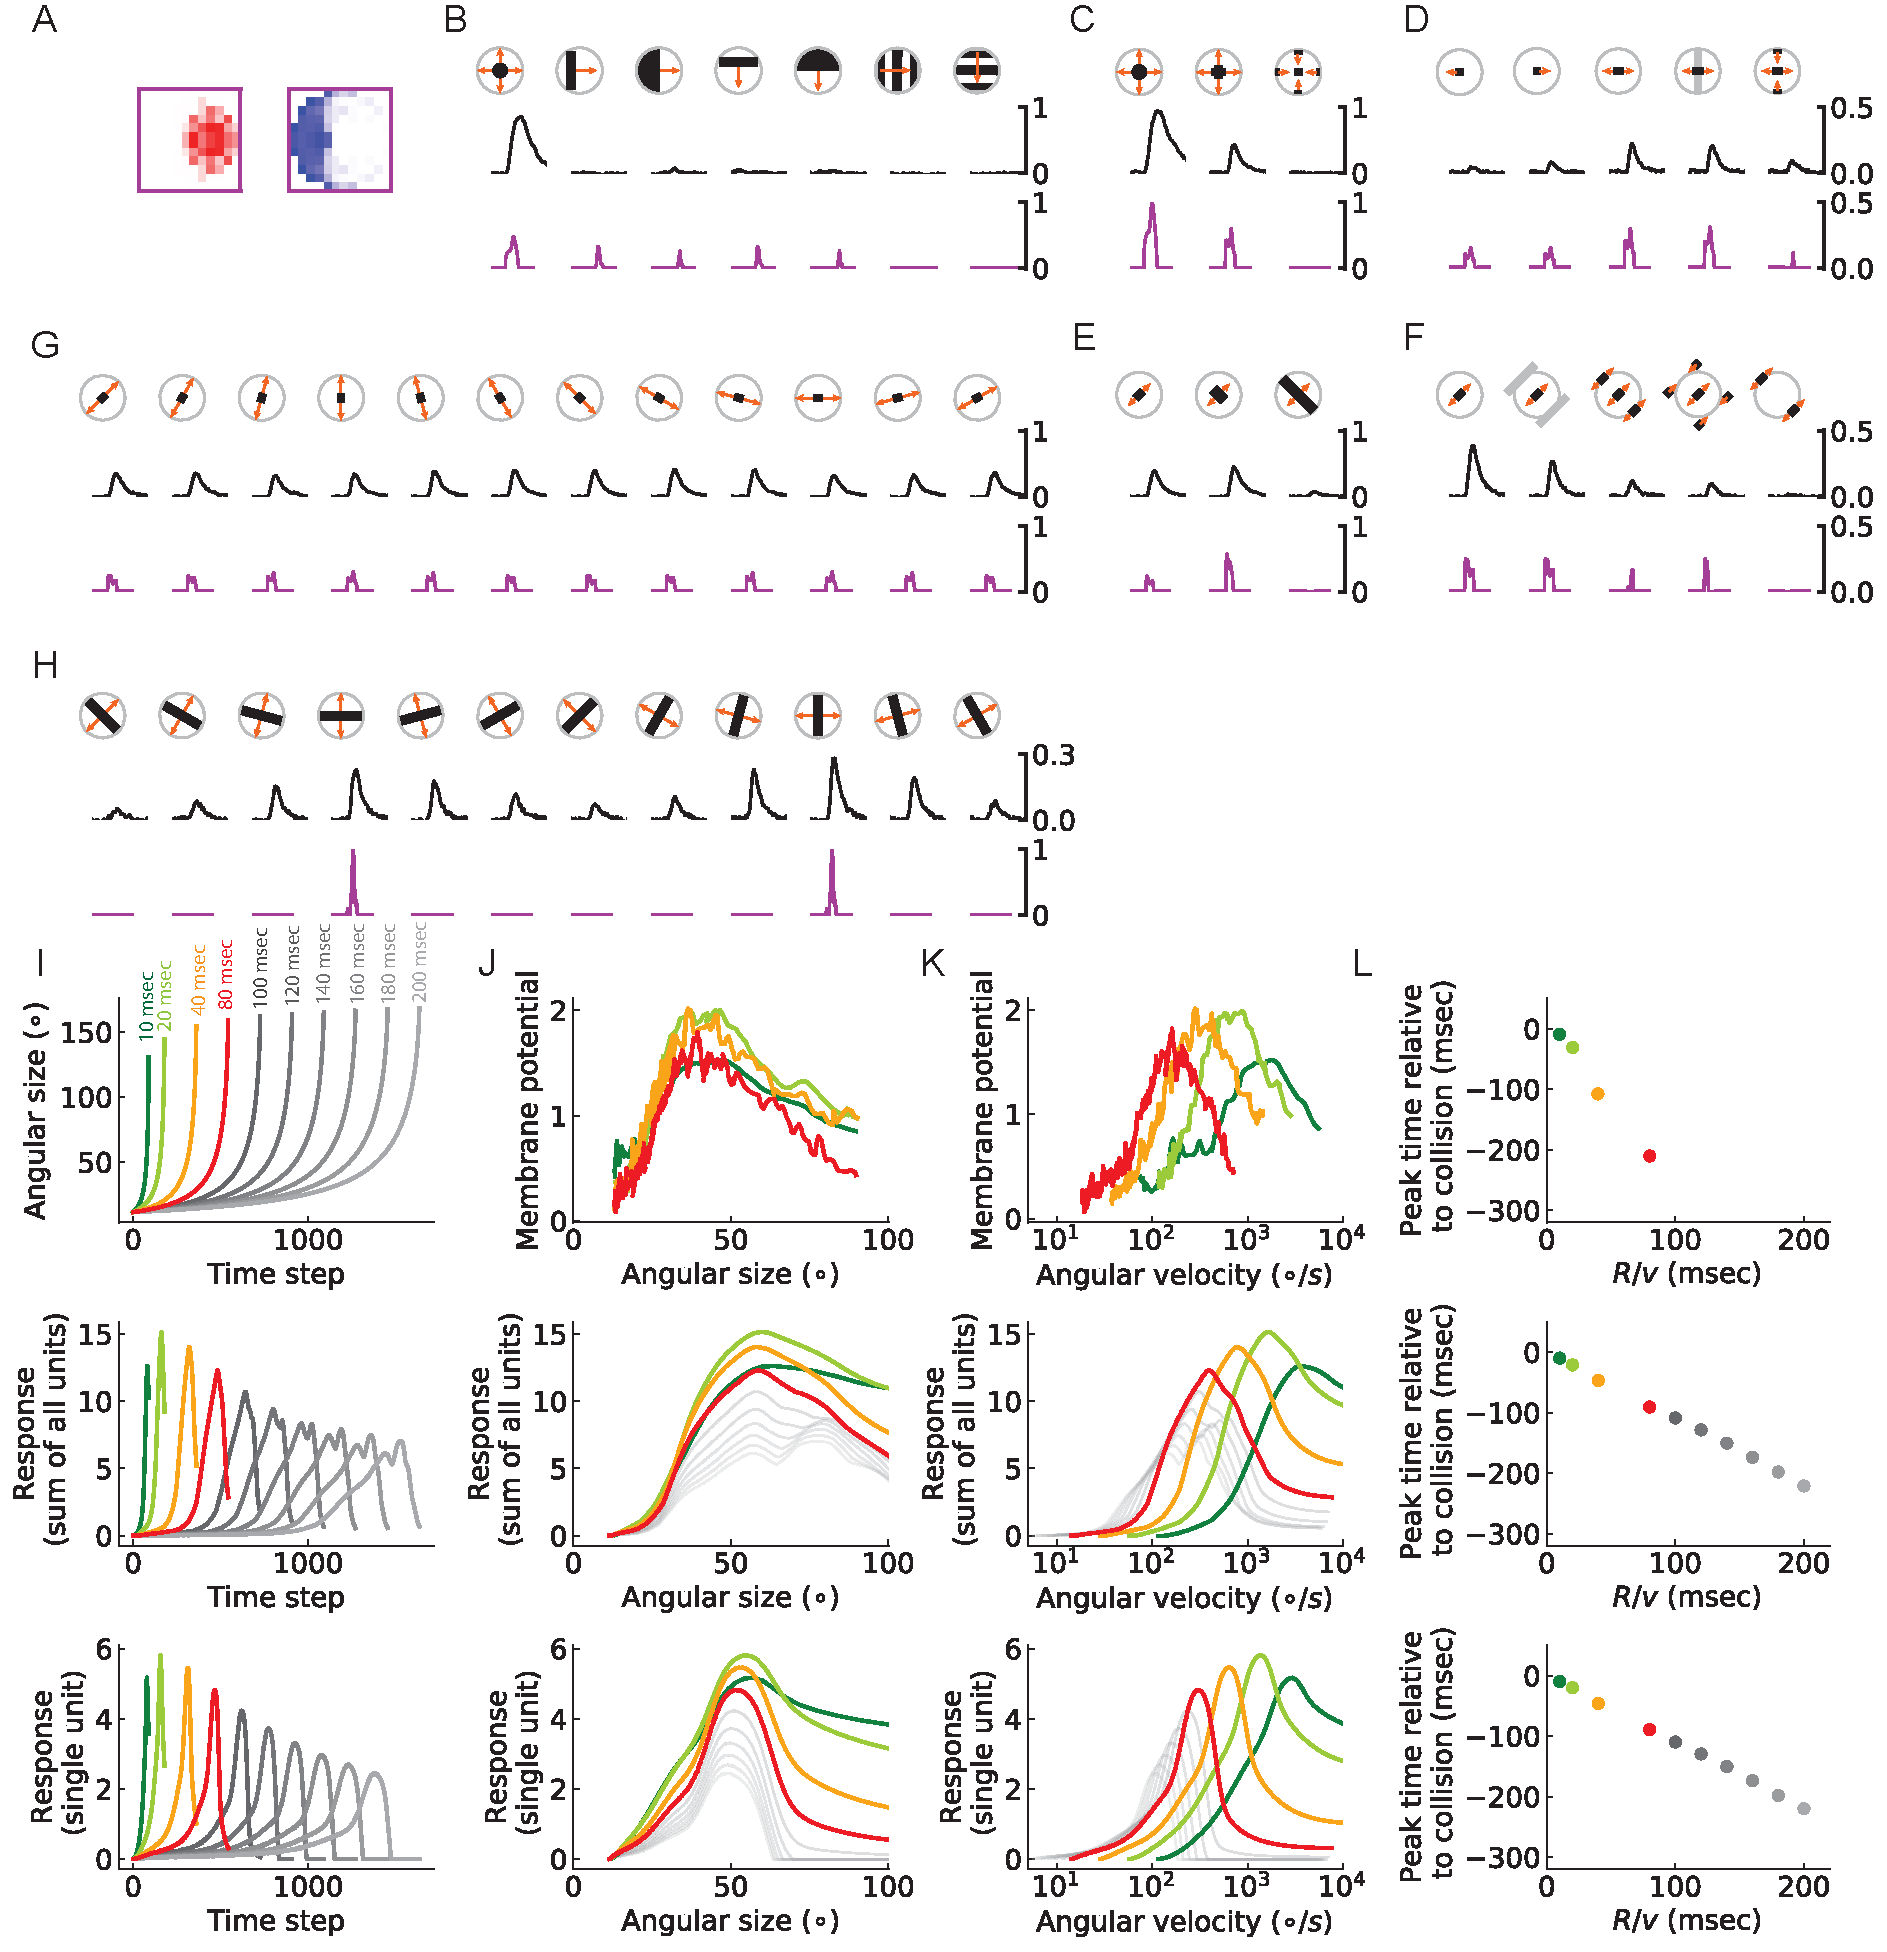
\includegraphics[width=0.8\linewidth]{figures/replication_paper.pdf}
\caption{Models trained on binary classification tasks exhibited similar responses to LPLC2 neurons observed in experiments. (A) Excitatory and inhibitory filters of the outward model with 256 units. (B-H) Comparisons of the responses of the model in (A) and LPLC2 neurons. Black lines: data \citep{klapoetke2017ultra}; magenta lines: model. Compared with the ones in the paper \citep{klapoetke2017ultra}, all the stimuli gadgets here except the ones in (B) have been rotated 45 degrees to the frame of reference that is attached to the fly head to match the cardinal directions of the LPLc2 neurons/units.}
\label{fig:replication}
%% If the optional argument in the square brackets is "none", then the caption *will not appear in the main figure at all* and only the full caption will appear under the supplementary figure at the end of the manuscript.
\figsupp[Same as in the main figure but for a different outward model obtained from the same training procedure.]{}{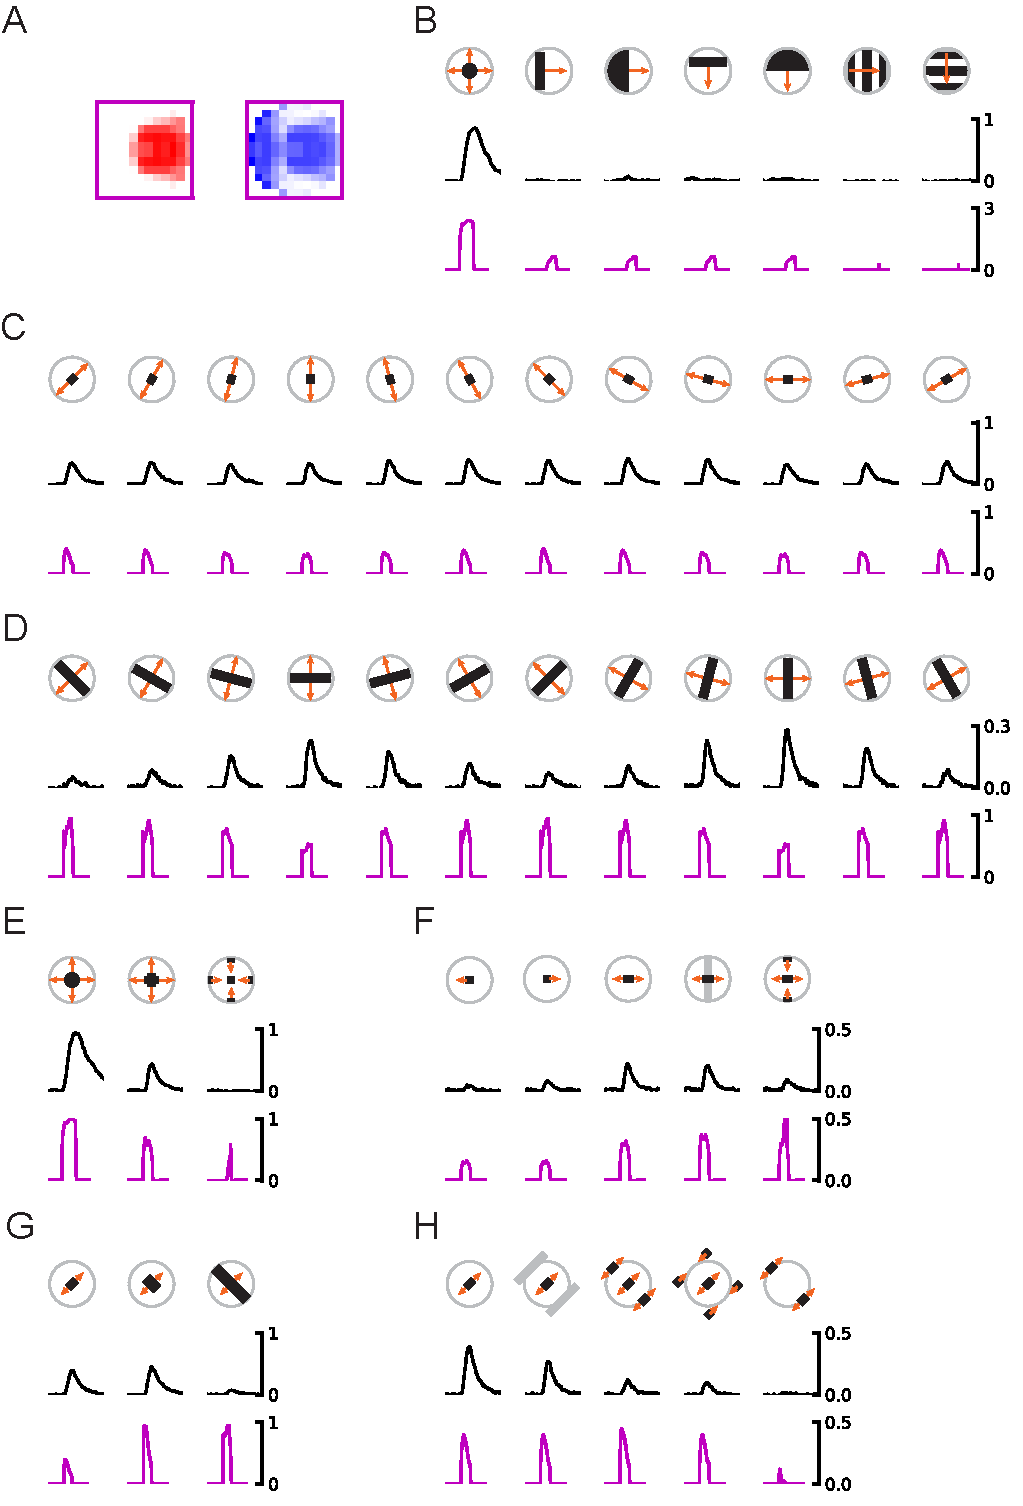
\includegraphics[width=0.8\linewidth]{sup_figures/replication_sup1_paper.pdf}}\label{figsupp:sf1_replication}
\end{figure}






\end{document}
